
\chapter{透过散射介质的光谱信恢复和空间信息恢复}
前面的章节中,我们已经介绍了散射成像的研究背景、发展现状及研究意义,并且对散斑的基本概念与特性进行了阐述,同时介绍了本章工作所依赖的基本物理特性
散斑的光谱多样性及光学记忆效应。

光谱成像已经发展多年,它在文成像到地球观测,以及生物医学成像等领域有着重要的应用前景。
然而,当光线通过生物组织或毛玻璃等混浊介质时,会被强烈散射并扩散成复杂且杂乱的散斑图案,
这使得利用目标的光谱信息和空间信息变得困难。虽然,目标的空间信息和光谱信息保存在所获取的散斑图案中,但是,如何有效地利用此类信息变得极为挑战。
伴随着对散射特性的深入研究,波前调制技术、光学传输矩阵和散斑相关等技术在透过散射介质成像方面有着重要的应用。然而,波前调制技术需要较长的波前优化过程,且耗时较长,
有效地选取恰当的反馈信号对该技术的应用起着决定性的作用。与此同时,波前调制技术的实现往往需要利用光学或声学探针,对聚焦信号实现定位或者引导,才能够有效
地实现聚焦。光学传输矩阵技术需要对散射介质的传输矩阵进行测量,记录特定输入信号及其对应的输出信号,
通常难以在非入侵的情境下实现成像工作,如:生物成像等。2012年,意大利学者J.Bertolotti等人提出了基于“光学记忆效应”(OME)的散斑相关成像方法,
通过相关的方式从散斑数据中获取目标的傅里叶振幅,进一步利用相位恢复算法从傅里叶振幅中实现目标的傅里叶相位信息恢复,最终,实现隐藏目标的空间信息重建。
然而,此方法需要对入射激光光源进行多角度扫描,其成像质量与角度扫描的数量密切相关。2014年,以色列学者O.Katz等人受到天文成像方法的启发,对散斑
相关成像方法进行改进,实现了单帧散斑的透过散射介质成像。透过自相关的方法从单帧散斑获取目标的傅里叶振幅信息,然后利用相位恢复算法恢复相应的傅里叶相位信息,
进而恢复目标的空间信息。即使能够实现对隐藏目标的散斑成像,但是恢复目标的光谱信息仍极其困难。在光谱域,当单色光通过散射介质后,其散斑图像的强度分布与
与入射光的波长相关。2013年,B.Redding等人提出了基于介质光谱传输矩阵光谱重建方法。此方法将不同单色光通过散射介质的散斑作为该波长的指纹,并将不同的光谱
指纹存储在矩阵中,称为光谱传输矩阵。当有未知光谱信息的光源输入系统时,只需要记录其相应的散斑并对其进行求解,便可以实现对未知光源的光谱信息恢复。在随后的
发展中,许多学者将此光谱重建的方法的应用扩展到无序光子晶体、多模光纤和散射介质等。然而,此方法只能对目标信息的光谱信息进行恢复,无法实现目标的结构信息的恢复。

在本章中,我们首先介绍了基于光谱传输矩阵的光谱信息恢复方法和基于光学记忆效应的散斑相关成像方法的基本原理,并对其进行了仿真复现;其次,我们对两种方法进行了
结合,设计了一个双臂系统实现透过散射介质实现光谱成像。对于我们的系统,一个臂用于通过光谱传输矩阵的方式实现光谱信息重建,另一臂用于通过散斑关成像方法实现目标结构信息重建。
最后,我们进行了了实验,验证了该系统能够有效地实现目标光谱信息重建和空间信息重建。由于散射介质选择的多样性,该系统在低造价的成本下,实现了对目标结构和光谱信息的重建。

\section{基于光谱传输矩阵和散斑相关成像方法的原理介绍}
图\ref{fig:3.1}所示为本章所要描述的透过散射介质的光谱信息和结构信息恢复的结构示意图。输入光通过光学准直器照明目标,然后又分束镜将来自于目标的光束分为两束,
一束进入光谱测量臂,另外一束进入结构信息重建臂。在光谱臂中,光束被由单模光纤和透镜进行收集并准直,然后透过散射介质,被相机所探测。在成像臂中,光束直接照明散射
介质并透过散射介质,然后由相机接收散射后的散斑信息。在以下部分,我们分别对光谱重建的数学模型和散斑相关成像数模型进行描述。
\begin{figure}[htp]
	\centering
	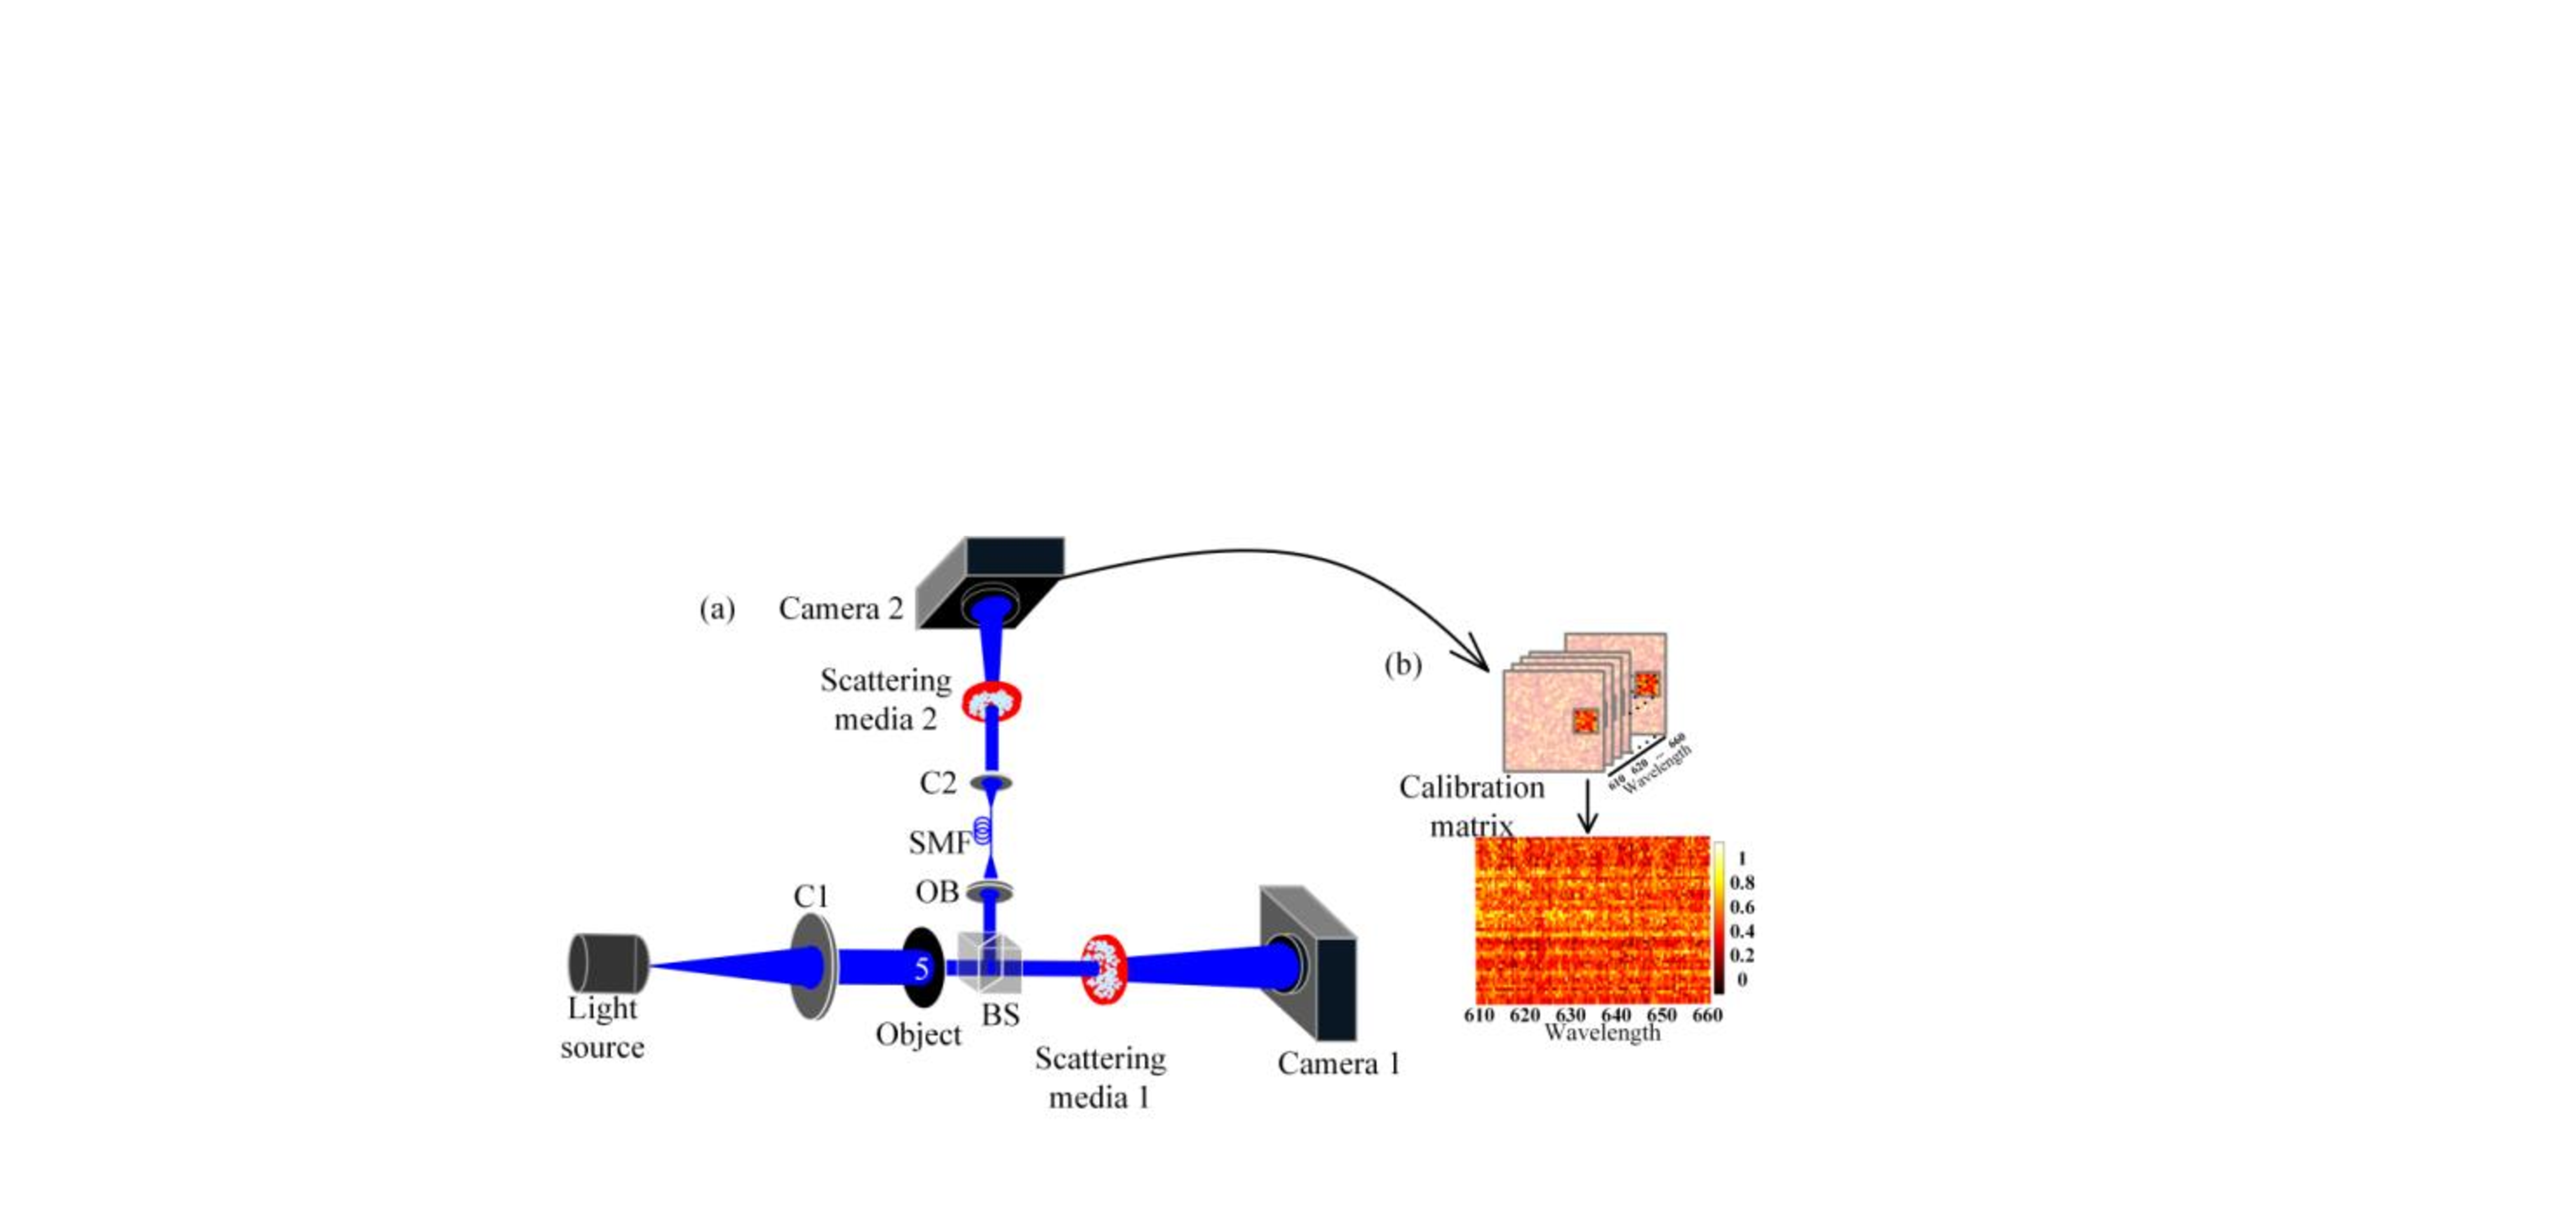
\includegraphics[scale=0.3]{Chapter3.FIG2.spectral_retrieval_model.pdf}
	\caption{透过散射介质的光谱信息和结构信息恢复的结构示意图}
	\label{fig:3.1}
\end{figure}

\subsection{基于光谱传输矩阵的光谱重建模型}
散斑图像中的强度分布取决于照明的角度、观察角度和入射光的波长等因素。在本小节中,我们只对入射光的波长变化进行讨论。首先,我们需要引入散斑的光谱多样性概念。如图\ref{fig:3.2}所示的系统中,照明光源与散射介质之间的距离为$d$,散射介质与相机之间的距离为$S_{0}$,
当特定波长以固定的角度照明散射介质时,散射光被位于介质后表面距离为$S_{0}$相机接收。在此,我们认为此类散射介质的散射效应随着波长的改变而变化。我们在惠更斯-菲尼尔近似条件下,
相机所接收的散斑图像可以表示为:
\begin{equation}
    E(r_{c},\lambda) = A\iint E(r_{o},\lambda)e^{\frac{ik}{2d}(r_{s}-r_{o})^{2}}Pup.(r_{s},\lambda)T(r_{s},\lambda)e^{\frac{ik}{2S_{o}}(r_{c}-r_{s})^{2}}\mathrm{d}{r_{o}}\mathrm{d}{r_{s}}
\label{eq:wavelength_diversity},
\end{equation}

其中,$k =2\pi/\lambda$,$r_{c}$、$r_{o}$和$r_{s}$分别表示相机平面,光入射面和散射介质平面的坐标,$Pup.(r_{s},\lambda)$为散射介质的孔径函数,$T(r_{s},\lambda)$为介质的散射作用。

我们固定公式(\ref{eq:wavelength_diversity})中的除波长以外测参数,分析波长改变对散斑分布的影响。首先,我们假设散射介质对于不同波长光引起的相位变化相同。在此假设下,波长的改变,会引起散斑图案的
空间缩放。其次,对于散射介质来说,其散射效应取决于波长。换而言之,对于不同波长入射光由散射介质引起的相位畸变不同,这样会导致所接受散斑图案分布发生变化,而非简单的缩放。但是对于实际应用中,往往两种
效应同时存在,或者往往更复杂,此种效应被称为散斑的波长多样性。同时我们也进行了相应的仿真,分析波长改变引起的散斑之间的相关系数的改变,仿真结果如图\ref{fig:3.3}所示。如何有效地利用散斑的波长多样性,将对散斑的波长信息利用有着重要的意义。

\begin{figure}[htp]
	\centering
	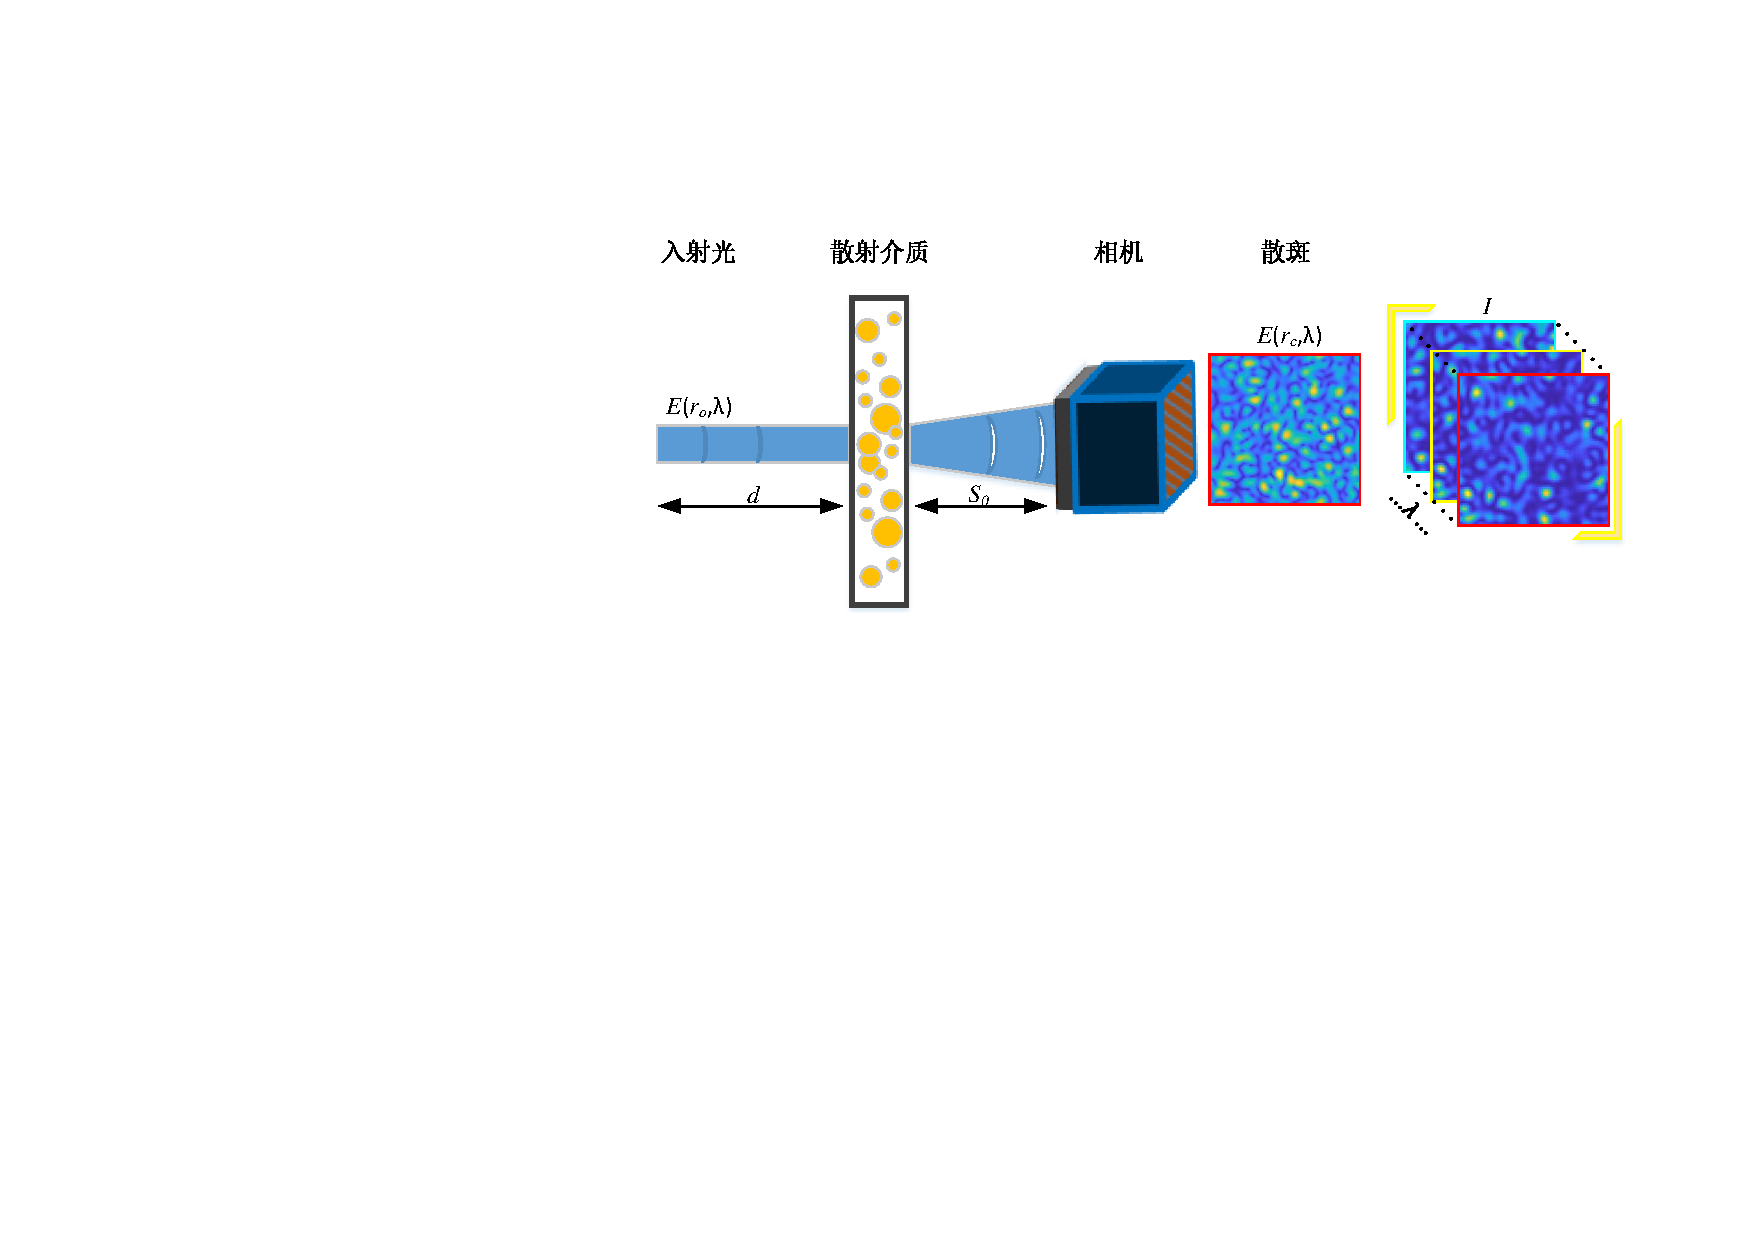
\includegraphics[scale=0.8]{C3.fig1.spectral_retrieval_model1.pdf}
	\caption{散斑的波长多样性}
	\label{fig:3.2}
\end{figure}

如果我们对散射介质的光谱指纹进行标定,并将不同的光谱指纹存储在矩阵中,此矩阵称为光谱传输矩阵。在此情况下,在获得未知光源照射散射介质所获得的散斑后,是否能够光谱传输矩阵和此散斑对未知光源的光谱信息进行重建?
答案是可以。如图\ref{fig:3.1}b所示,将不同的光谱指纹转换行向量,并按照光谱信息存储在矩阵$\Phi$中,当获取未知光源对应的散斑时,同样将其转换为向量$I$。所以,其输入信号的光谱$S$可以表示为:$I={\Phi}S$,对矩阵进行
左乘求逆,并求出最小二乘解:$S={\Phi}^{-1}I$。值得强调的是,该光谱重建方法不仅局限于对于以标定的单色光谱信号进行重建,同时也可应用于连续光谱信号。
上述的光谱重建问题可以为更普遍的最小化问题:$s_{0}=\arg{\min_s \| I -{\Phi}S \|_2}$,其中$\|  \|_2$表示$l-2$范数,$s_{0}$表示所重建的光谱信号,可以通过采用不同的最小化优化算法解决此问题。
\begin{figure}[htp]
	\centering
	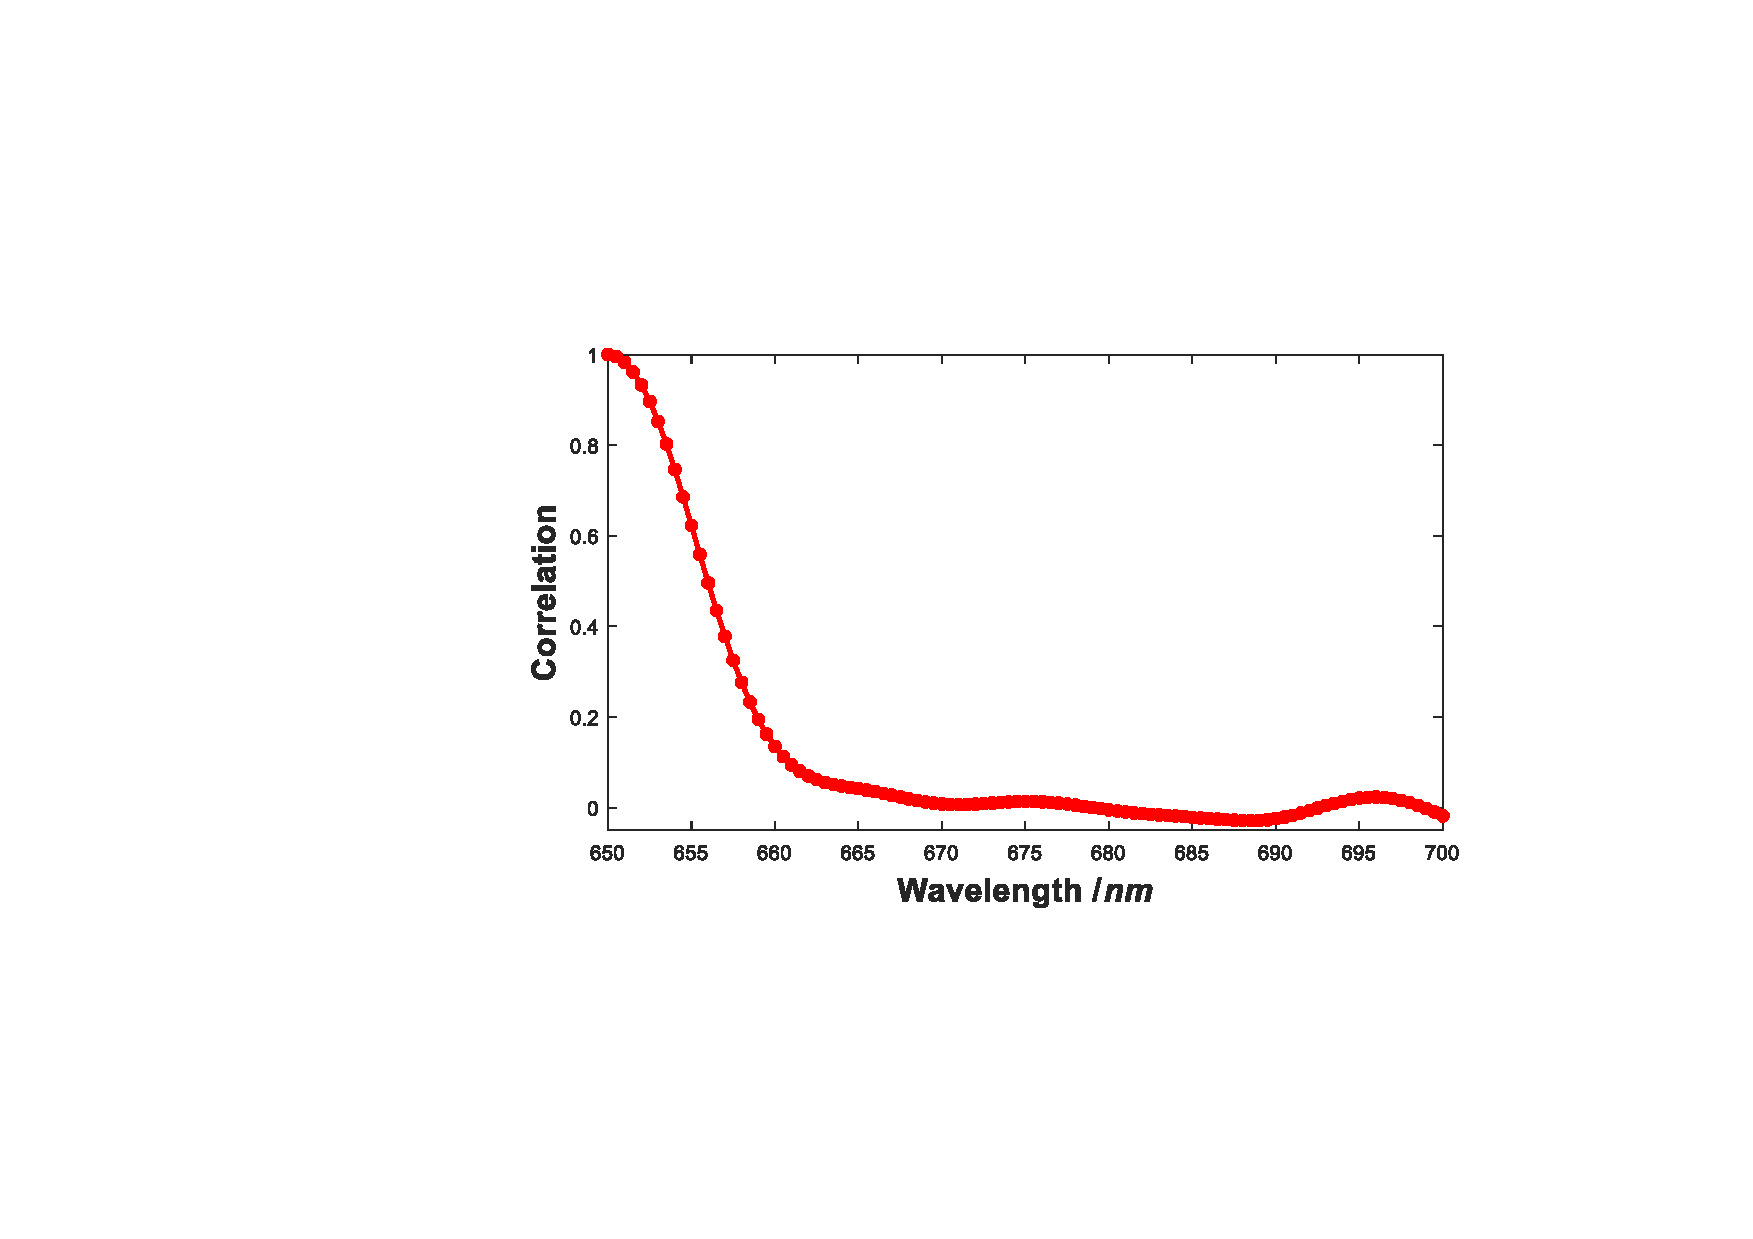
\includegraphics[scale=0.5]{C3.fig3.spectral_correlation_speckle.pdf}
	\caption{散斑的相关系数}
	\label{fig:3.3}
\end{figure}
\subsection{基于光学记忆效应的散斑相关成像模型}
图\ref{fig:3.4}所示为基于光学记忆相应的散斑相关成像基本模型,目标与散射介质之间的距离为$d$,散射介质与相机之间的距离为$S_{0}$。目标由空间非相干光源照明提供照明,目标所发出的光经过
散射介质后,被相机所接收。当物体位于此散射介质的OME范围之类时,由于OME范围内的点扩散函数具有空间平移不变性,相机所探测到的散斑可以表示为:
\begin{figure}[htp]
	\centering
	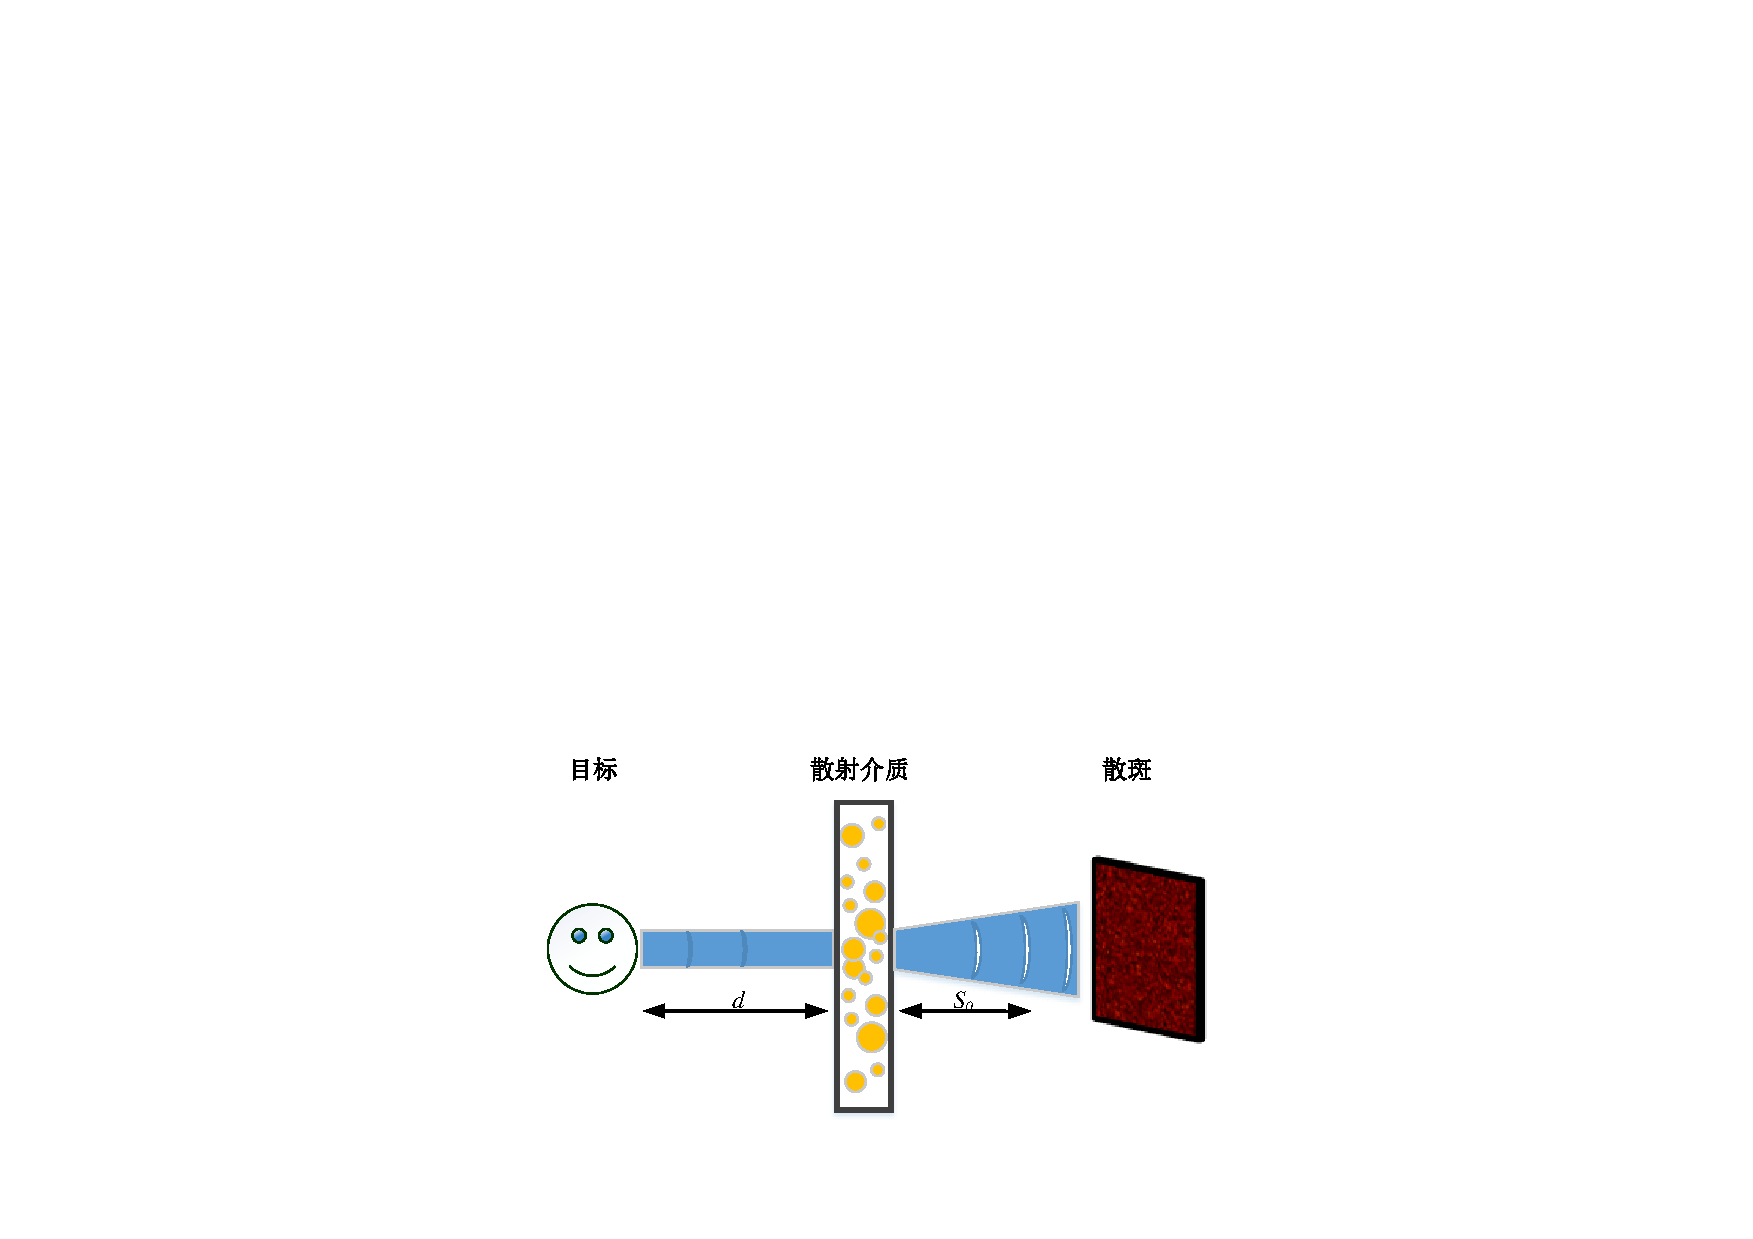
\includegraphics[scale=0.7]{C3.fig4.imaging_model.pdf}
	\caption{散斑相关成像模型}
	\label{fig:3.4}
\end{figure}

\begin{equation}
    I = O*S
\label{eq:speckle_autocorrelation_imgaing}
\end{equation}其中,$*$为卷积运算,$I$表示相机散斑,$O$表示目标和$S$表示系统的PSF。

透过散射成像的数学模型的理论基础如下,目标可以分解为不同的点源目标,当不同的点源目标为与散散介质的光学记忆效应范围之内时,不同点源目标所对于系统的响应函数可以近似看作不同的散斑在空间的平移。假设所有的点源目标被同时
点亮时,相机所接收到的图像为不同点源目标所对应散斑的非相干叠加。所以,光学记忆效应范围内目标的非相干成像模型可以卷积的形式进行表示:$I = O*S$。但是值得注意的是,大多是散射介质的光学记忆效应范围是有限的,当目标的尺寸超过光学记忆效应范围时,
此时卷积模型需要加入新的限制条件。成像系统的放大率$M$取决于物距$d$和相距$S_{0}$:
\begin{equation}
    M = \frac{d}{S_{0}}
\label{eq:magnification_imgaing_system}
\end{equation}
成像系统的分辨率$\Delta \theta $可以表示为:
\begin{equation}
    \Delta \theta   \propto \frac{\lambda}{nD}
\label{eq:angleresolution_imgaing_system}
\end{equation}
其中,$\propto$表示正比关系,$\lambda$为照明光源的波长,$n$表示光经过散射介质后的介质折射率,$D$表示散射介质的有效孔径,孔径的大小可以通过加载光阑实现控制。

上述部分中,我们具体描述了基于光学记忆效应的散射基本成像模型,如公式(\ref{eq:speckle_autocorrelation_imgaing})所示,当获得散斑图像后如何恢复图像将在接下来部分进行描述。
意大利学者J.Bertolotti,以色列学者O.Katz等人先后基于散斑自相关的特性,提出了基于光学散斑自相关的图像重建算法。当相机获得散斑图案后,散斑的自相关可以表示为:
\begin{equation}
\begin{aligned}
    I \bigstar I  = (O*S) \bigstar (O*S) \\
		              =  (O \bigstar O)*(S \bigstar S)
\end{aligned}
\label{eq:autocorelation_equation}
\end{equation}
其中,$\bigstar$表示自相关运算。由公式(\ref{eq:autocorelation_equation})可知,散斑的自相关可以表示为目标的自相关与系统PSF自相关的卷积。当前成像系统PSF的自相关$(S \bigstar S)$可以近似
为$\delta$函数。所以,公式(\ref{eq:autocorelation_equation})可以简化为:
\begin{equation}
\begin{aligned}
    I \bigstar I  = (O \bigstar O)+C
\end{aligned}
\label{eq:autocorelation_equation_1}
\end{equation}
其中,$C$表示自相关计算中的背景常数项。通常,在自相关图像恢复中,我们需要将背景常数项进行剔除。如果对公式(\ref{eq:autocorelation_equation_1})左右两边同时进行傅里叶变换,我们会获得什么呢?
庆幸的是,我们获得了以下公式:
\begin{equation}
\begin{aligned}
    \mathcal{F}(I \bigstar I)  = \mathcal{F}(O \bigstar O)
\end{aligned}
\label{eq:autocorelation_equation_2}
\end{equation}
公式(\ref{eq:autocorelation_equation_2})继续可以简化为:
\begin{equation}
\begin{aligned}
    \mid \mathcal{F}(O) \mid = \sqrt{\mathcal{F}(O \bigstar O)}\\
		               = \sqrt{\mathcal{F}(I \bigstar I)}
\end{aligned}
\label{eq:autocorelation_equation_3}
\end{equation}
根据公式(\ref{eq:autocorelation_equation_3})可知,我们可以通过计算的方式从散斑图像中获得隐藏目标的傅里叶振幅信息,当获得目标的傅里叶振幅信息之后,仍然缺失的是目标的傅里叶相位信息。
图像恢复问题已经被转换为依据傅里叶振幅信息恢复傅里叶相位信息的问题,幸运的是此类相位恢复问题在相位中属于常见问题。相位恢复算法不是本节研究的重点,因此在本节中,我们将简要介绍在后续图像恢复中所用到
的基本相位恢复算法,其算法流程如图\ref{fig:3.5}所示。该类型相位算法的核心思想为:步骤一,获得傅里叶振幅信息$\mid \mathcal{F}(O) \mid$,随机的给予随机的傅里叶相位初始值$\phi$,并对其进行傅里叶变换,进而将信号转换至空间域,并获得目标的初始猜测$g_t(x,y)$;
步骤二,对信号$g_t(x,y)$进行傅里叶变换,将其变换至频域$G_t(k_x,k_y)$,将$G_t(k_x,k_y)$的傅里叶振幅部分替换为$\mid \mathcal{F}(O) \mid$,保留其傅里叶相位信息,此时的信号表示为$G^{\prime}_t(k_x,k_y) =\mid \mathcal{F}(O) \mid e^{i\phi (k_x,k_y)}$;步骤三,对信号$G^{\prime}_t(k_x,k_y)$进行再一次傅里叶变换,将其转换至空间域,
根据目标信号的稀疏性及非负性,设置约束条件,对信号进行处理,此时获得的信号表示为:$g^{\prime}_t(x,y)$;步骤四,用$g^{\prime}_t(x,y)$替换为步骤一中的$g_t(x,y)$,并重复步骤二至步骤四,直至满足约束条件停止此相位恢复程序。

\begin{figure}[htp]
	\centering
	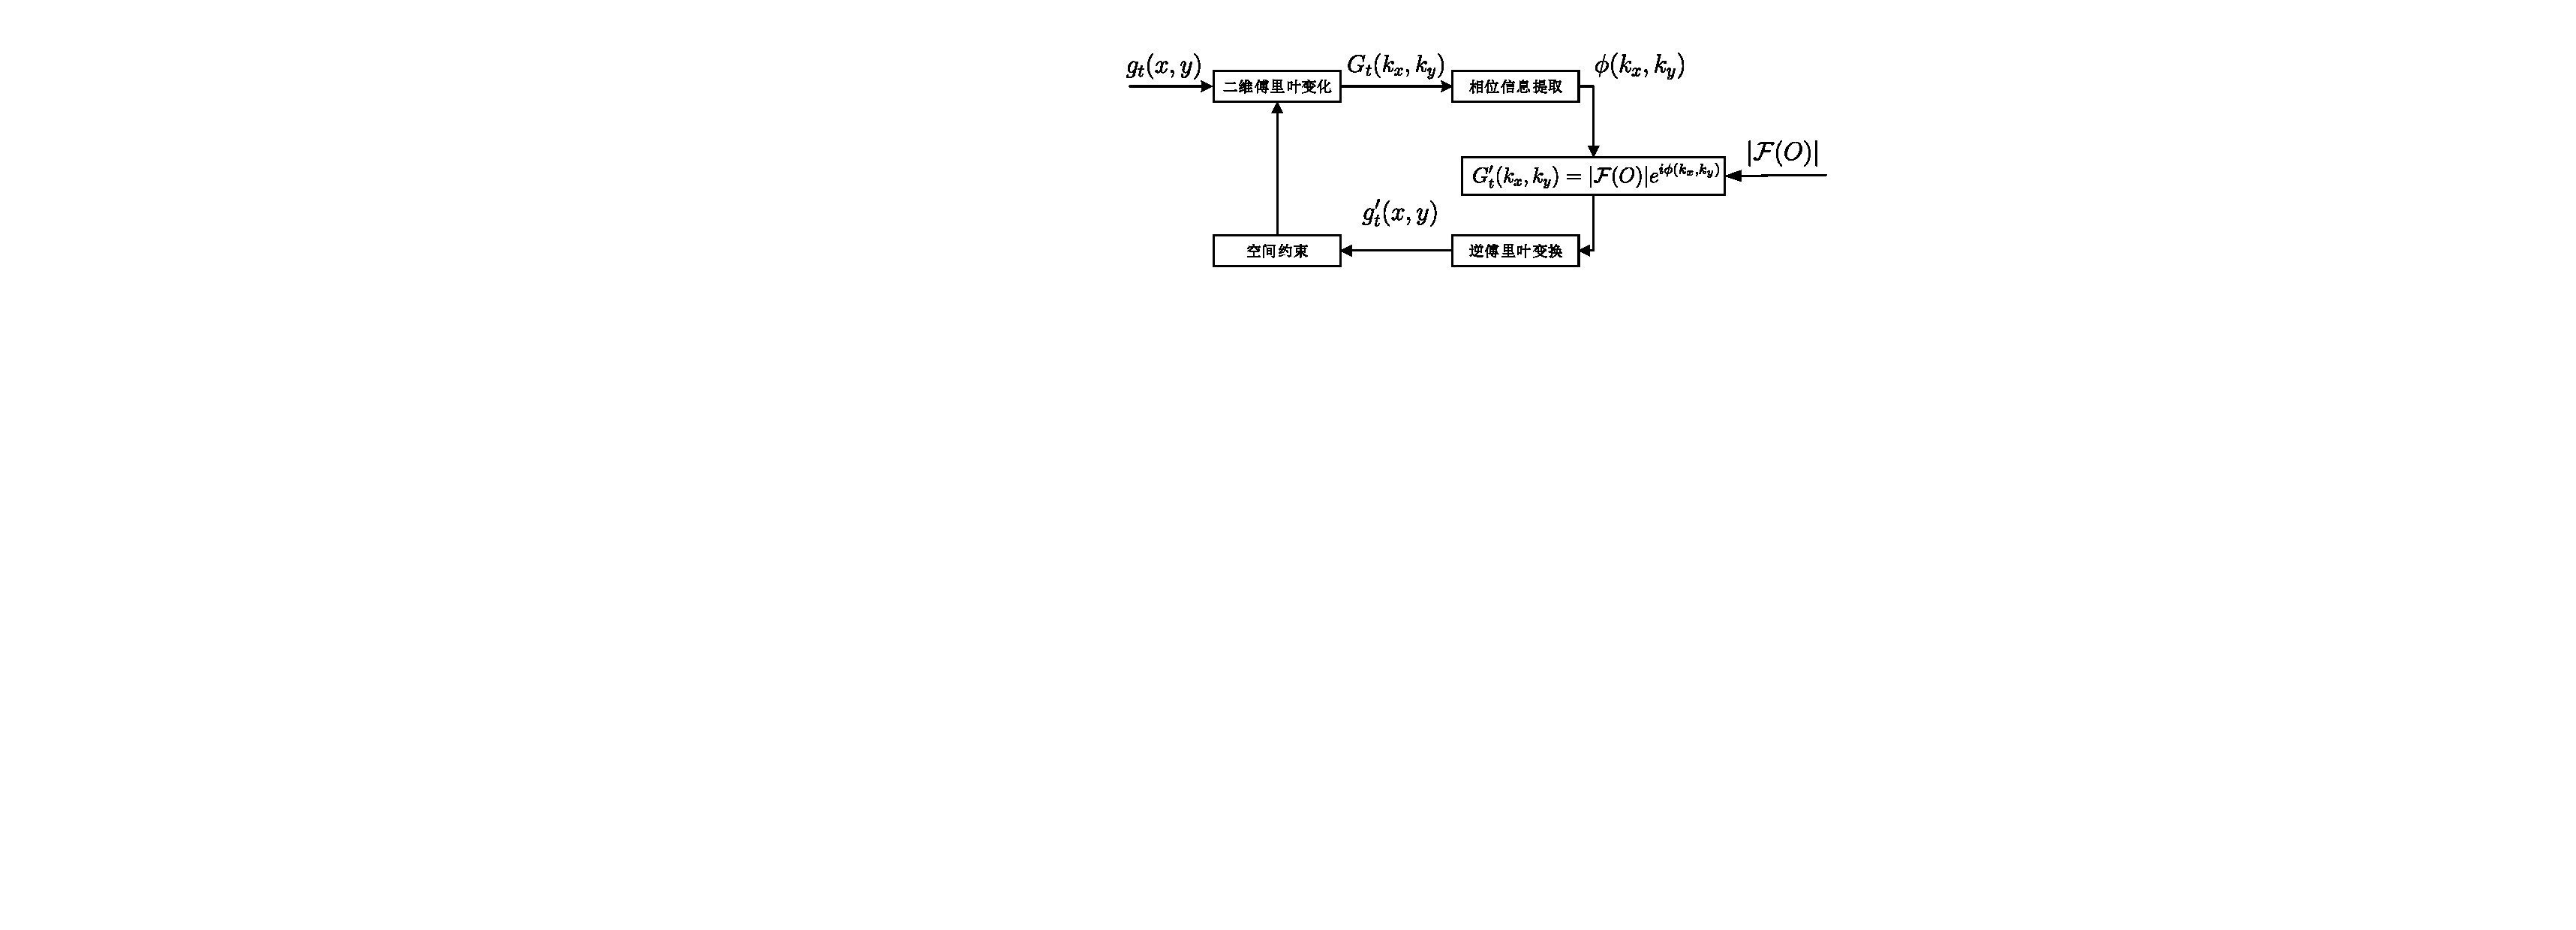
\includegraphics[scale=0.7]{C3.fig5.phase_retrieval_model.pdf}
	\caption{基本相位恢复流程图}
	\label{fig:3.5}
\end{figure}
在实际的应用中,不同相位恢复算法在空间域采用不同的约束条件。例如,混合输入输出(Hybrid Input-Output,HIO)算法的约束条件如公式(\ref{eq:constrain_HIO})所示,误差减小(Error
reduction,ER)算法的约束条件如公式如公式(\ref{eq:constrain_ER})所示。
\begin{equation}
\begin{aligned}
 g_{t+1}(x,y) =
		  \begin{cases}
		    g_{t}^{\prime}(x,y)   &   (x,y)\notin\Gamma\\
		    g_{t}(x,y)-\beta g_{t}^{\prime}(x,y) & (x,y)\in\Gamma
		  \end{cases}
\end{aligned}
\label{eq:constrain_ER}
\end{equation}
其中,$\beta$为算法收敛性的参数,$\Gamma$为满足约束条件的集合。

\begin{equation}
\begin{aligned}
 g_{t+1}(x,y) =
		  \begin{cases}
		    g_{t}^{\prime}(x,y)   &   (x,y)\notin\Gamma\\
		    0  & (x,y)\in\Gamma
		  \end{cases}
\end{aligned}
\label{eq:constrain_HIO}
\end{equation}

\section{光谱信息恢复及散斑自相关成像方法仿真验证}
上述部分,我们对光谱信息恢复及散斑相关成像的基本原理继续了介绍,因此在本小节中,我们对上述的原理进行数字仿真验证及实验验证。
B.Redding等人在文献中以对基于光谱传输矩阵的光谱重建方法进行了详细的理论分析,所以在此我们对该方法进行简单的数值分析以及仿真验证。光谱重建的仿真原理如图\ref{fig:3.2}所示,
分别记录不同波长输入光对应的散斑$I_\lambda$,并将$I_\lambda$存储在光谱传输矩阵中。然后,输入未知光谱$s_{o}$记录其对应的散斑信号$I_{o}$,根据公式$s_{0}=\arg{\min_s \| I_{o} -{\Phi}S \|_2}$对光谱$s_{0}$进行求解。
在散斑图像重建方面,首先我们生成对应的PSF,根据公式(\ref{eq:speckle_autocorrelation_imgaing})生成目标对应的散斑,然后利用上述的散斑自相关成像方法进行图像恢复。

透过散射介质光谱成像的仿真参数如表\ref{table:1.1}所示,仿真结果如图\ref{fig:3.6}所示,第一行,为成像臂在不同波长光照明情况下,相机1所探测到的散斑;第二行,为光谱臂在不同光谱不同波长光照明下,相机2所接收到的散斑;
第三行,利用散斑相关成像方法所恢复的目标图像;第四行,利用光谱传输矩阵方法所恢复的光谱信息。从仿真结果图\ref{fig:3.6}第一列至第三列可以看出,当输入光为窄带宽的光源时,该光谱成像方法能够有效地恢复图标的空间信息和光谱信息。从图\ref{fig:3.6}第四列
可以看出,当照明光源为宽谱光源时,该光谱成像方法仍然能够有效的重建目标的光谱信息和空间信息。

\begin{table}[!htbp]
\begin{center}
\caption{仿真参数}
\label{table:1.1}
\begin{tabular}{|c|c|}
\hline
\textbf{仿真参数} & \textbf{数值}\\
\hline
光谱范围 & $600 \sim 650 nm$ \\
\hline
光谱采样间隔 & $0.5  nm$\\
\hline
空间采样间隔 & $12.0 \mu m$ \\
\hline
散射介质维度 & $600 \times 600$ \\
\hline
\end{tabular}
\end{center}
\end{table}

\begin{figure}[htp]
	\centering
	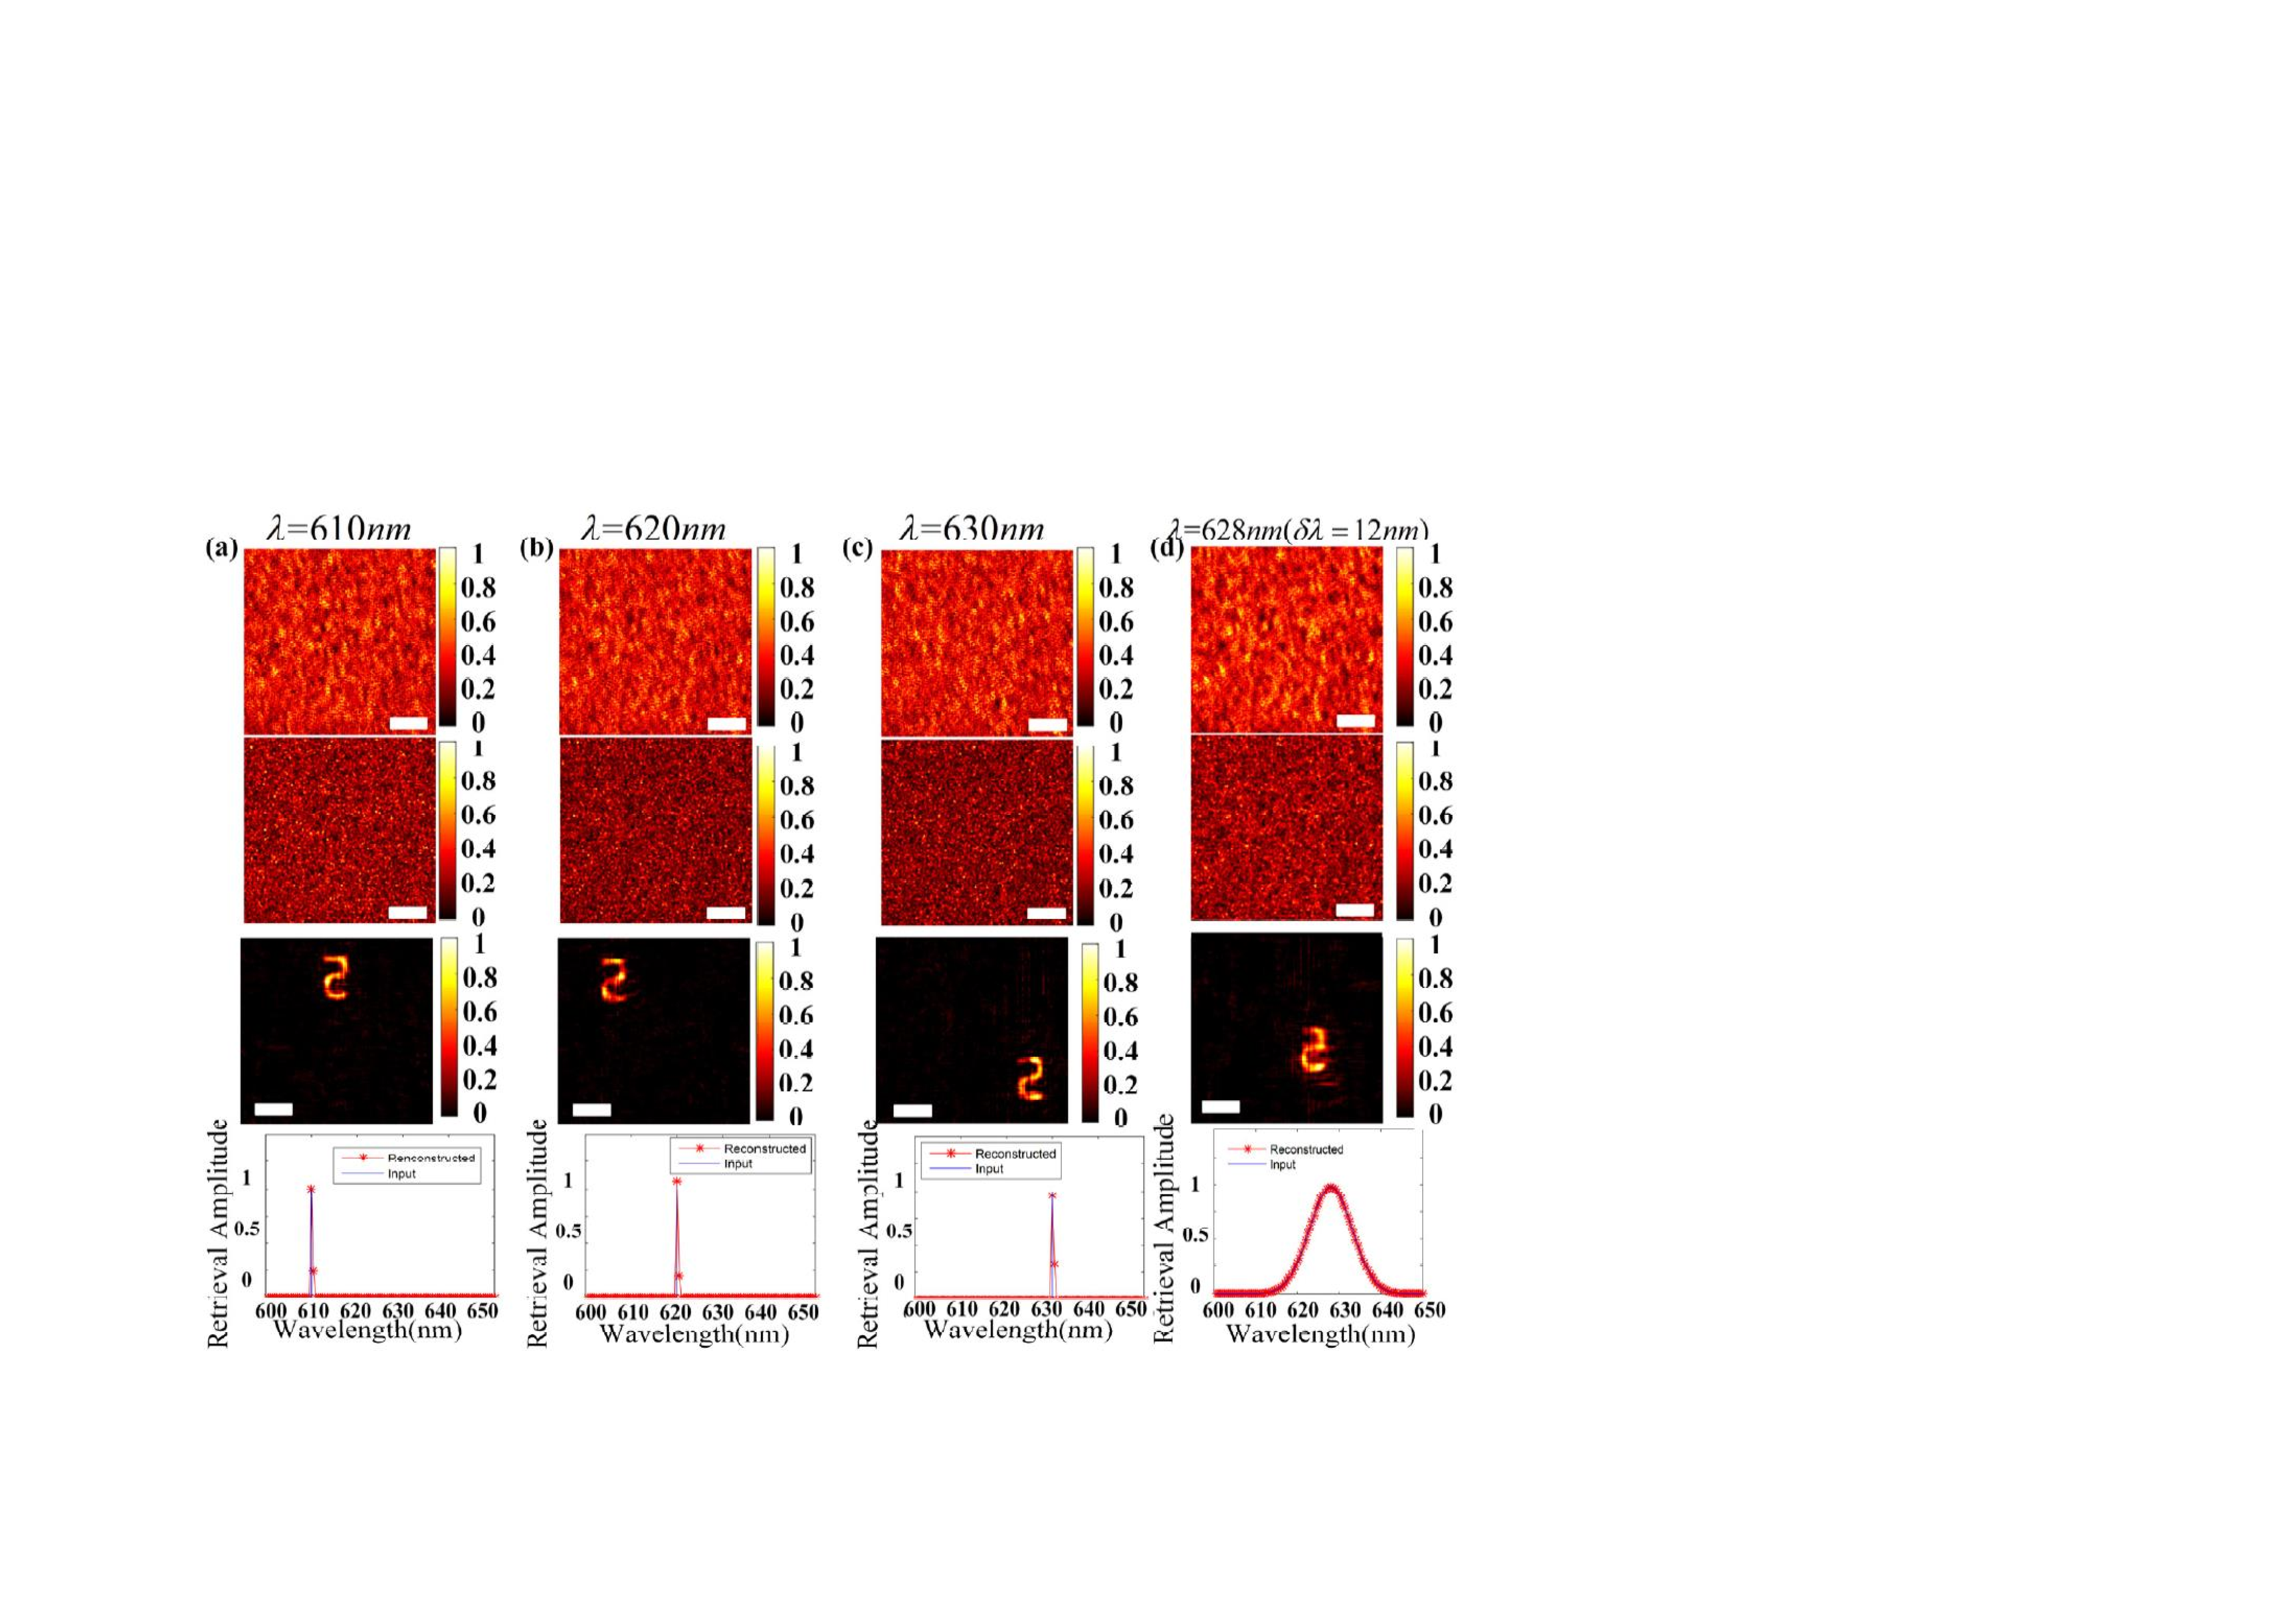
\includegraphics[scale=0.45]{C3.fig6.simulation_results.pdf}
	\caption{仿真结果}
	\label{fig:3.6}
\end{figure}

我们所用到的基于光谱传输矩阵的光谱重建方法对于系统的噪声叫敏感,不同的重建优化方法在抗噪声方面有着不同表现。于是,我们通过在系统中引入不同功率的高斯噪声,并且进行了相应的重建,
计算重建信号与原始信号之间的相关系数,进而分析不同算法的抗噪性能。目前常用的重建算法有:吉洪诺夫正则化算法(Tikhonov regularization,TR)和凸优化算法(Convex Optimization,CVX)。
TR和CVX重建算法在不同噪声水平下的光谱重建结果如图\ref{fig:3.7}所示。从图中看可以看出,随着噪声从$50 dB$ 增加到 $35 dB$,TR和CVX两种重建算法的分别重建的光谱信号与原始信号之间相关系数接近于1,
但是当信噪比低于 $35 dB$时,CVX重建结果的相关系数大于TR重建的相关系数。因此我们相信,CVX在光谱重建方面的抗噪性能优于TR。

\begin{figure}[htp]
	\centering
	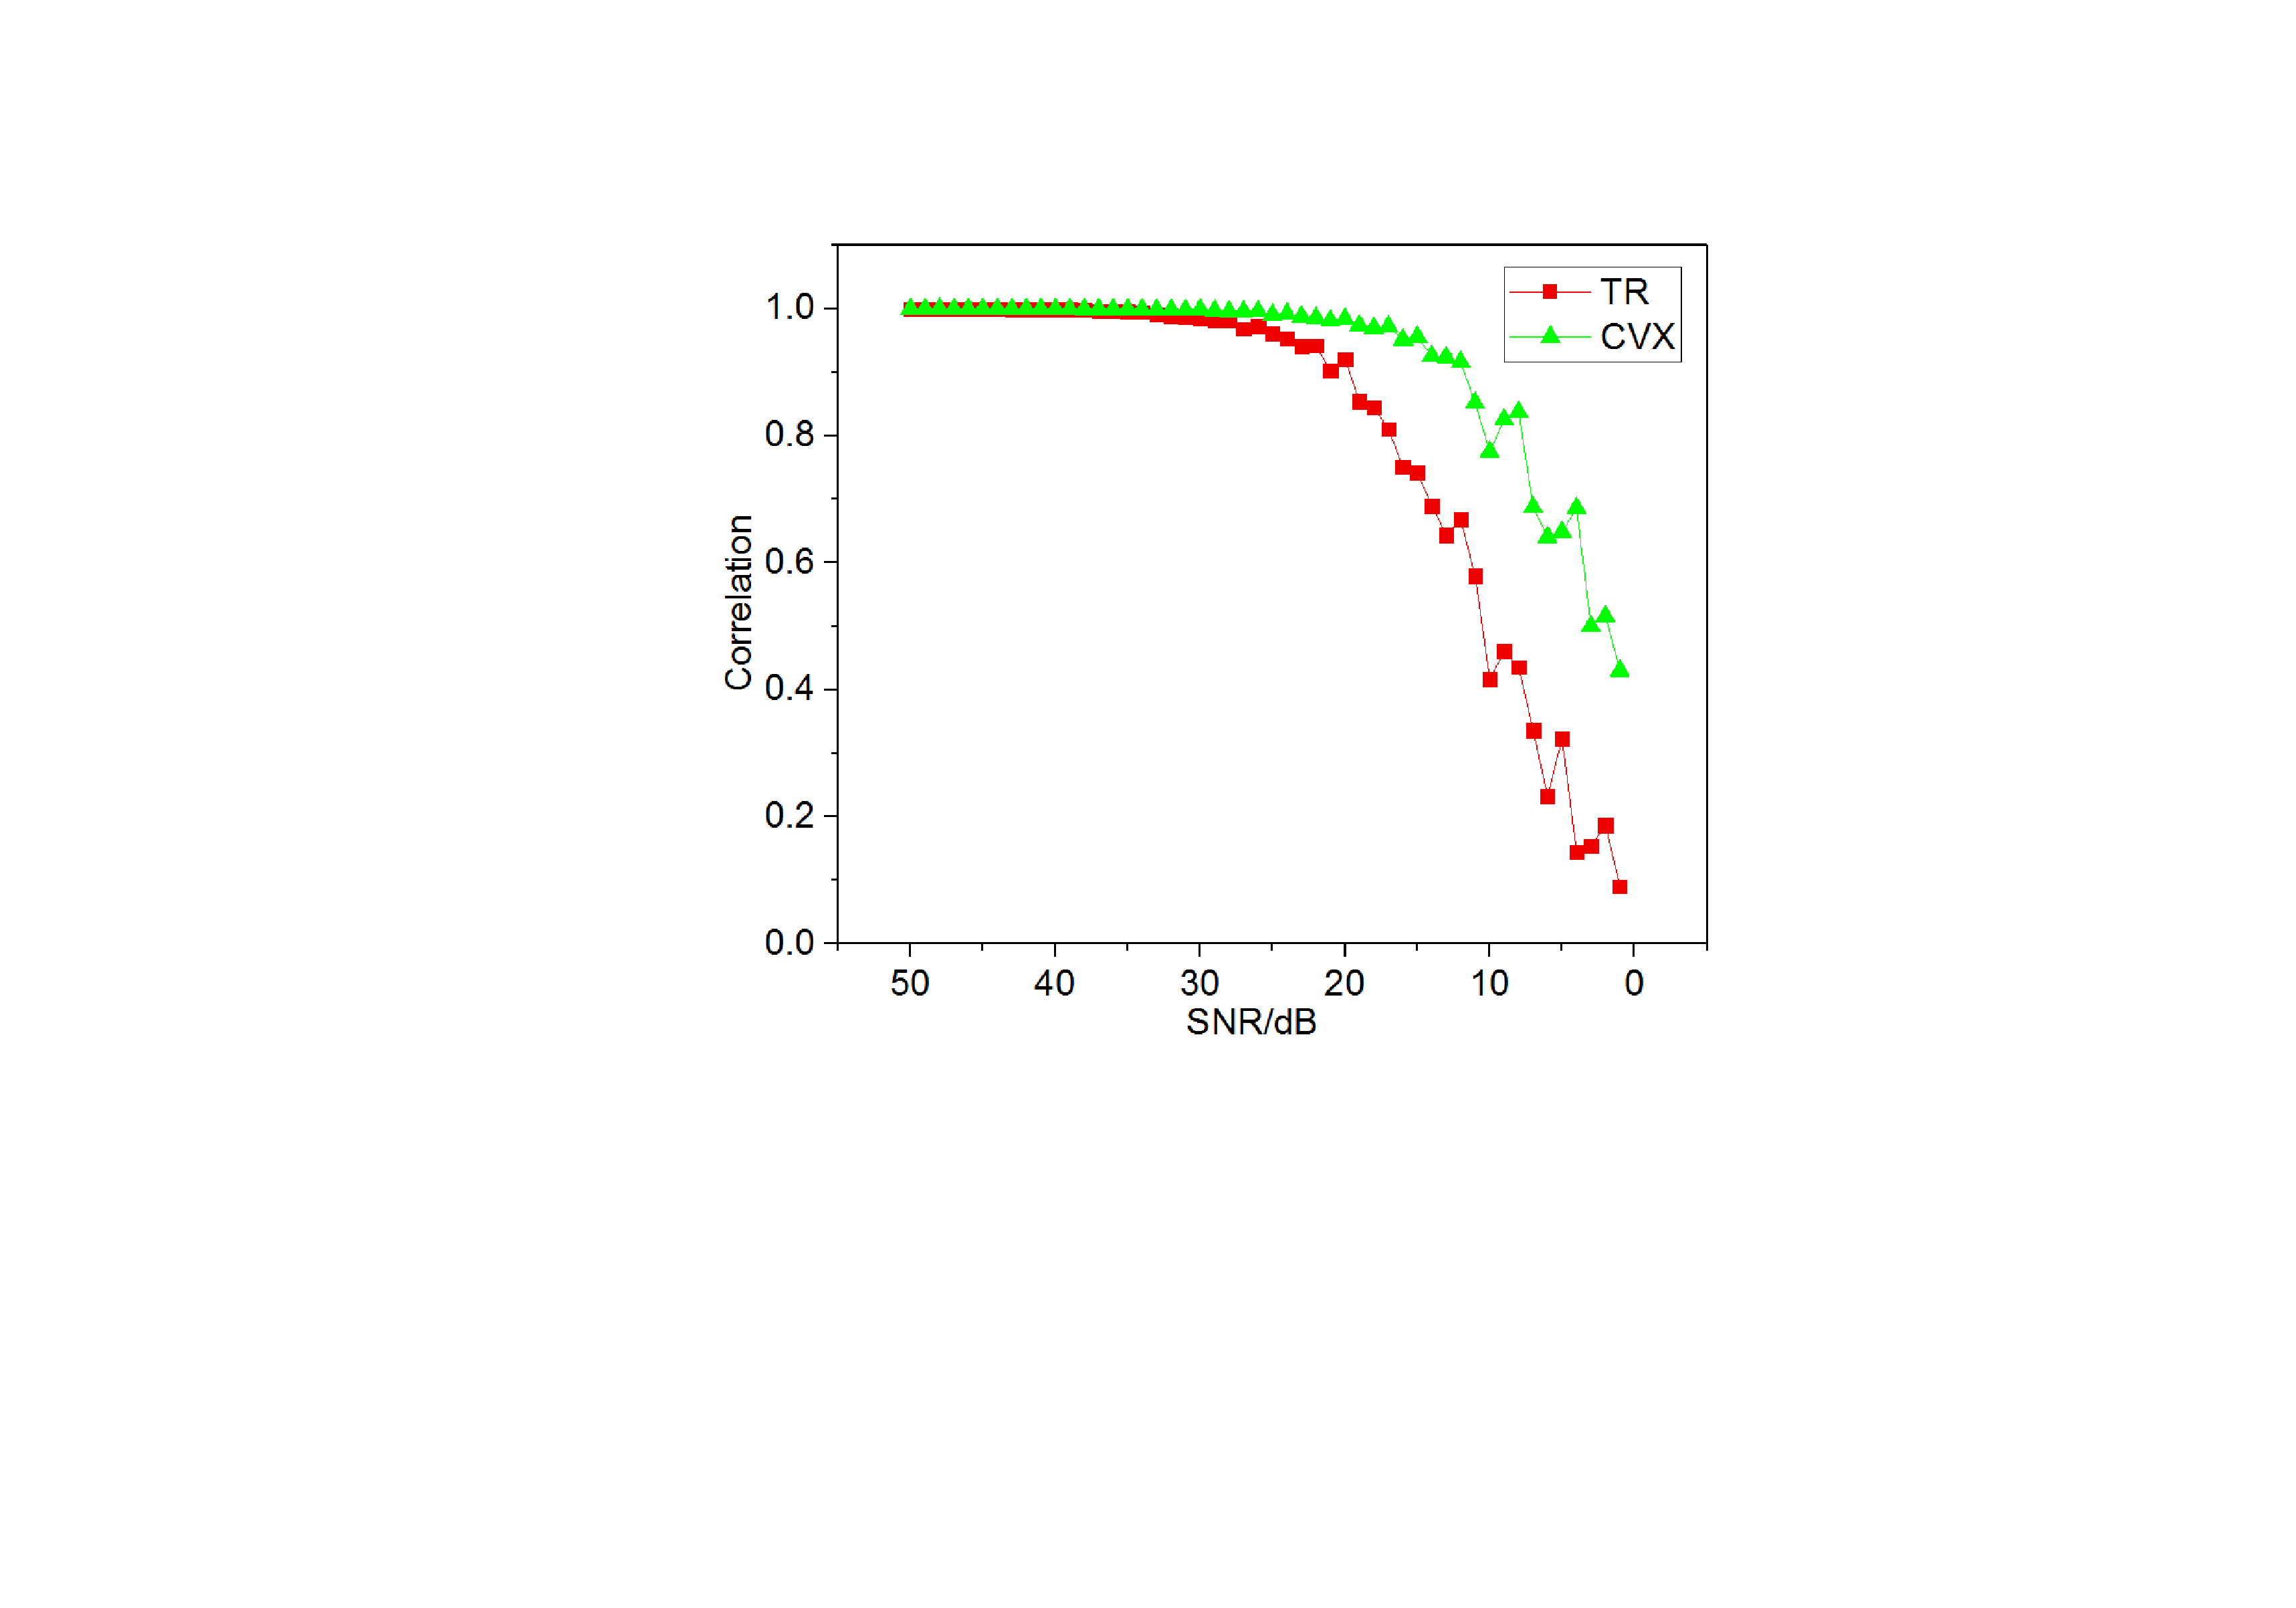
\includegraphics[scale=0.45]{C3.fig7.performance_under_fifferent_noise_levels.pdf}
	\caption{光谱重建算法的抗噪性能分析}
	\label{fig:3.7}
\end{figure}

\section{光谱信息恢复及散斑自相关成像方法实验验证}
实验光学装置如图\ref{fig:3.8}所示,\textcircled{1}:光源,\textcircled{2}:单色仪,\textcircled{3}:准直器,\textcircled{4}:分束器,\textcircled{5}:目标,\textcircled{6}:散射介质1,\textcircled{7}:相机1,\textcircled{8}:物镜,\textcircled{9}:单模光纤,
\textcircled{10}:透镜,\textcircled{11}:散射介质2和\textcircled{12}:相机2。
在实验中,我们使用厚度为$2mm$,颗粒度为$220$毛玻璃(Thorlabs,DG10-220)作为散射介质,目标为从分辨率测试靶标(1951USAF,Edmund Company)中选出的数字字符。
实验中,我们需要对光谱臂进行预标定,目的是获取光谱臂的光谱传输矩阵。在预标定过程中,我们利用来自氙气灯(Zolix, GLORIA-X500A)的作为照明光源,并用安道尔单色仪(Andor Spectrograph, Shamrock 500i)对照明光源进行光谱过滤,产生光谱分辨率
(Full Width Half Maximum,FWHM)为$1 nm$的可调光源。实验中使用相机是CMOS相机(AndorZyla5.5),像素尺寸为$6.5\mu m$和像素数为420万。
实验中,我们分别对$445 \sim 495nm$ 和 $610 \sim 660nm$两个光谱波段进行标定,预标定后的光谱传输矩阵分别如图\ref{fig:3.8}b和\ref{fig:3.8}c所示。
\begin{figure}[htp]
	\centering
	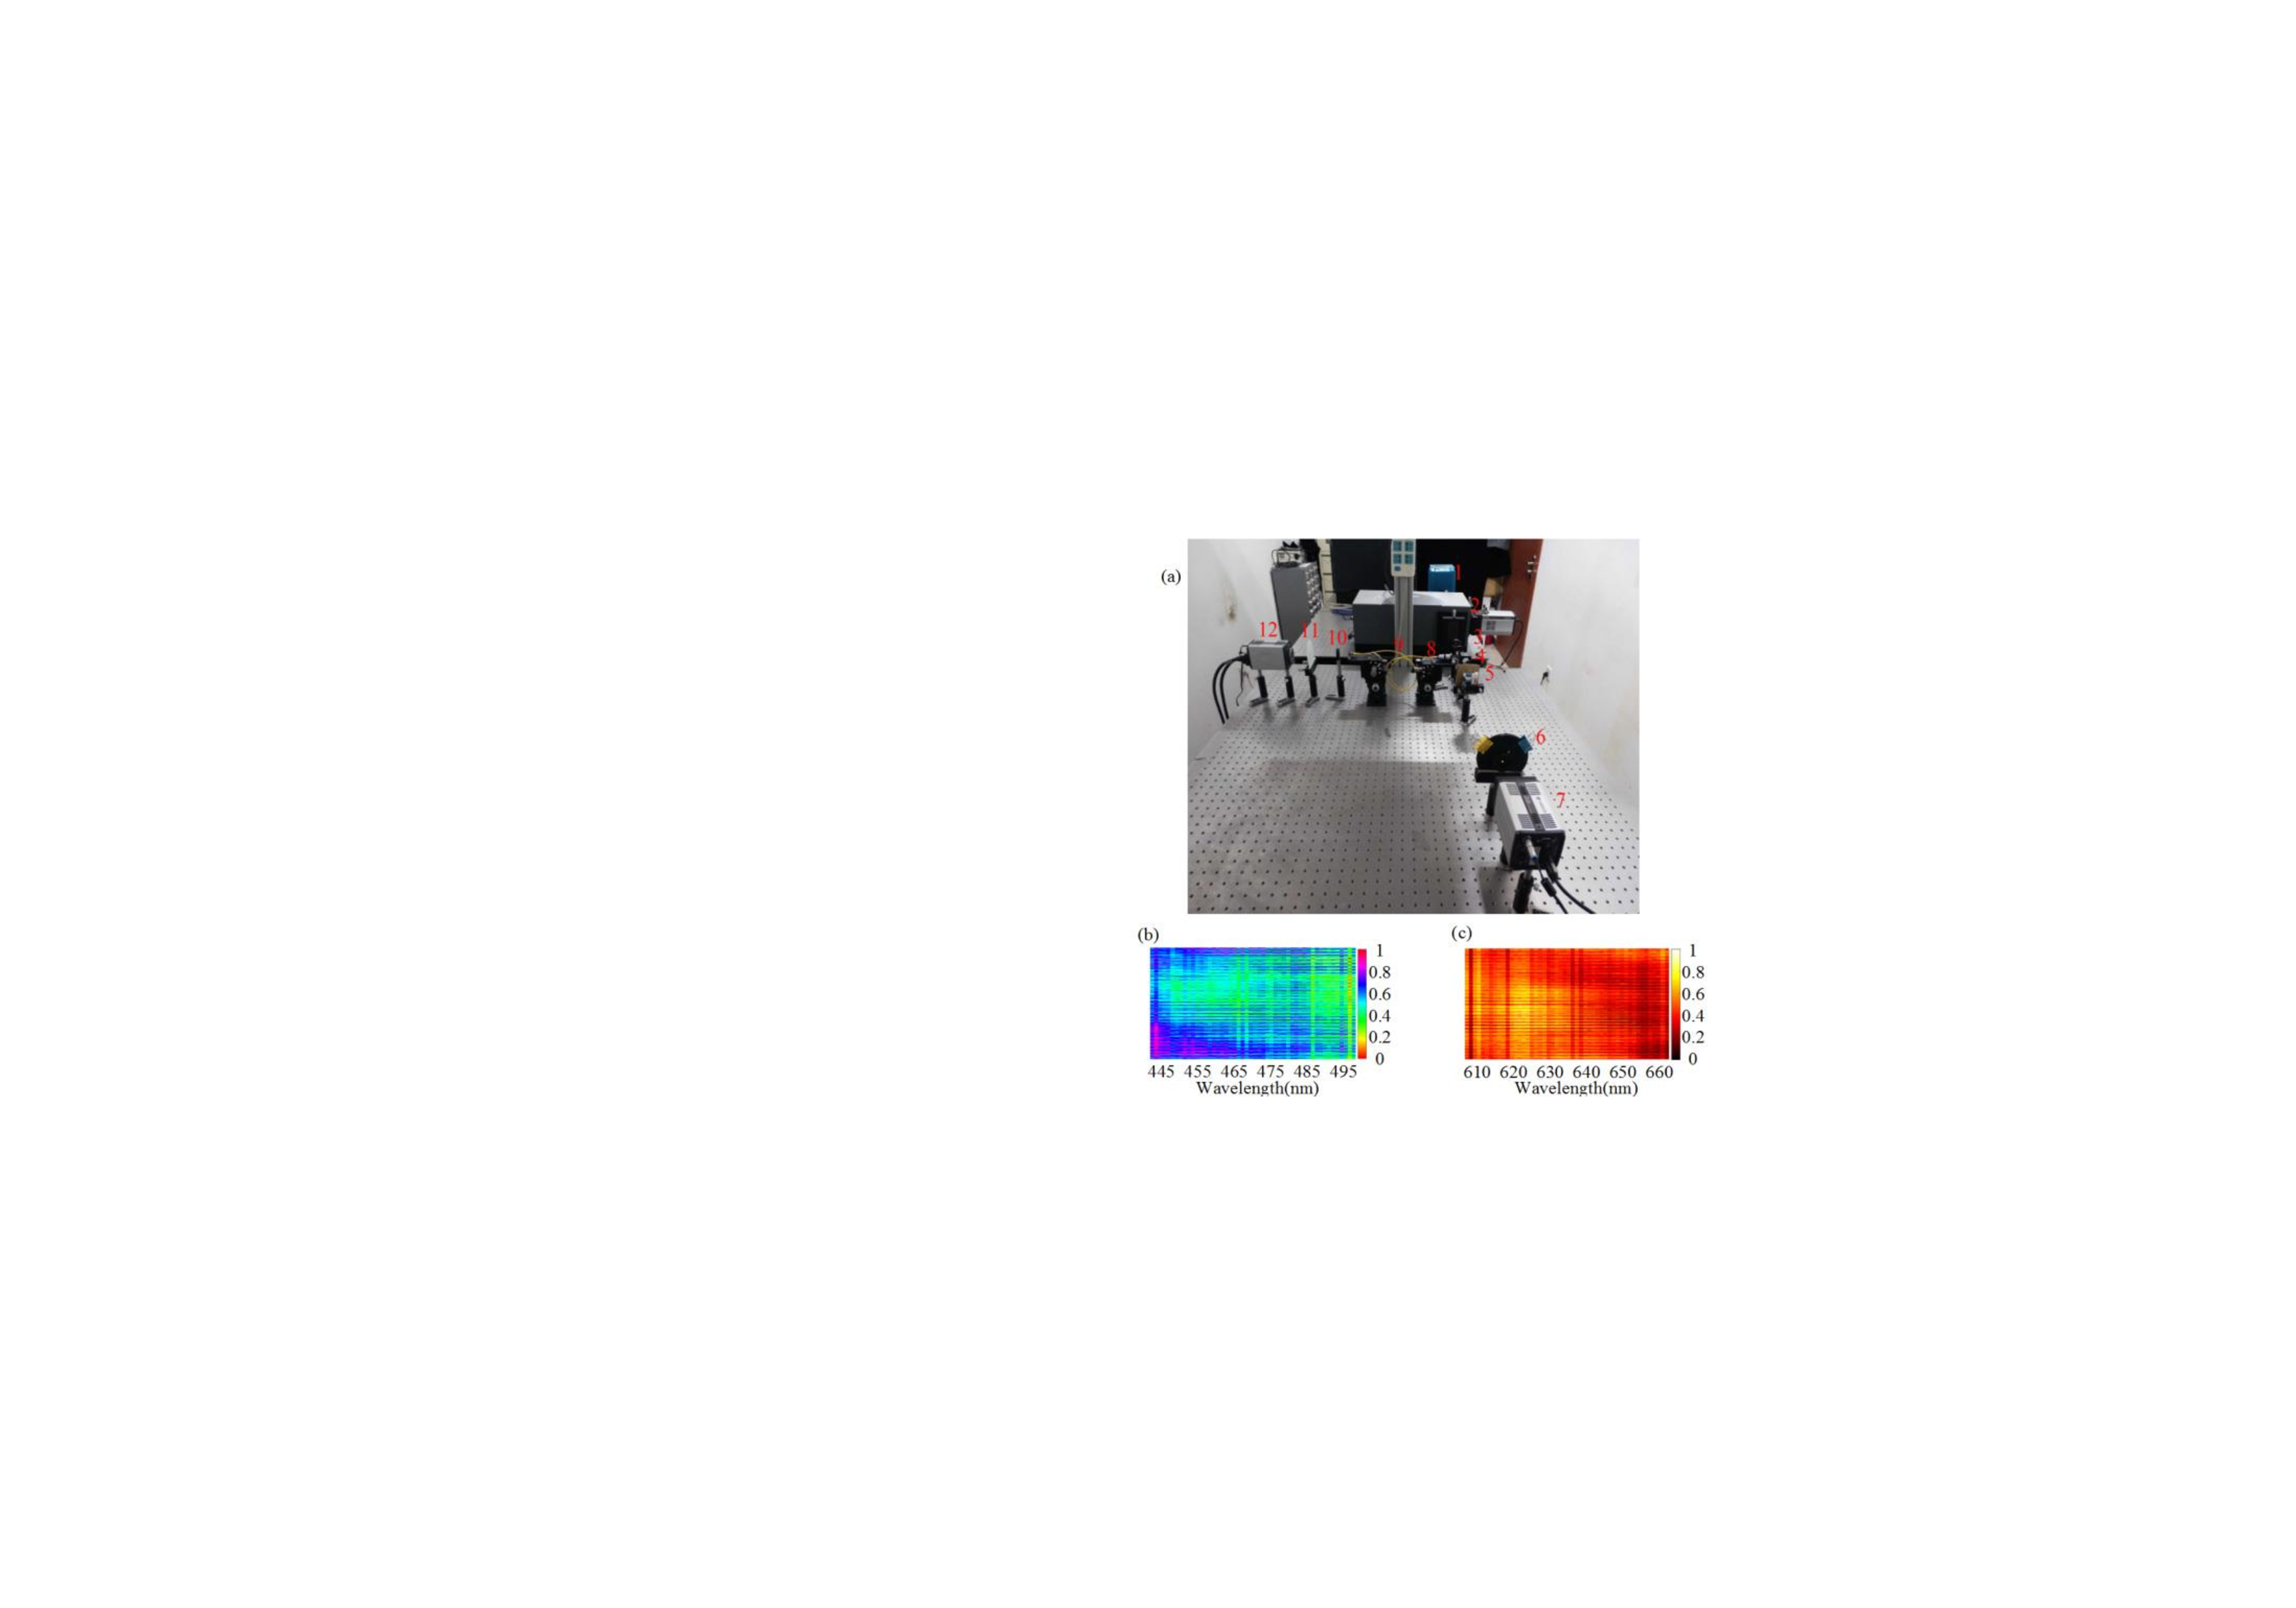
\includegraphics[scale=0.70]{C3.fig8.experimental_setup.pdf}
	\caption{光谱成像实验装置图}
	\label{fig:3.8}
\end{figure}
对于光谱标臂来说,我们利用物镜1和单模光纤对目标所发出的光进行收集,使用透镜对透过光纤后的光进行准直。这样的结构能够保证在我们的实验过程中,只需要对光谱臂进行的单次的光谱矩阵标定。
当完成光谱预标定后,我们采用了不同的目标对我们的系统进行测试,实验结果如图\ref{fig:3.9}所示。图\ref{fig:3.9}a和\ref{fig:3.9}b为利用单色光源照明时光谱信息恢复和目标空间信息重建结果,值得强调的是,此时我们使用的照明波长为已标定的光源波长。
我们的系统是否对未标定的连续光谱光源是否有效?们将在接下来部分进行详细分析。

\begin{figure}[htp]
	\centering
	
\includegraphics[scale=0.80]{C3.fig9.experimental_setup.pdf}
	\caption{光谱成像实验结果图}
	\label{fig:3.9}
\end{figure}

\subsection{光谱重建分析}
对于我们的照明光源可以分为两种:窄带光源和宽谱光源。为了验证光谱重建的有效性,首先我们利用已标定的光谱波段作为照明光源,进行光谱重建的有效性验证。光谱标定矩阵如图\ref{fig:3.8}b所示,在$445 \sim 495nm$光谱范围内,利用可调光源分别产生单色光源对目标进行照明,
波长分别为:$459nm$、$466mn$、$473nm$和$481nm$,并对其光谱信号进行重建,重建结果如所示\ref{fig:3.10}a。从图\ref{fig:3.10}a可以看出,在于单色光源照明时,我们能够有效的重建照明的光源的光谱信息。同理,在$610 \sim 660nm$光谱范围内,进行了相同的实验,实验结果
如图\ref{fig:3.10}b所示。


\begin{figure}[htp]
	\centering
	
\includegraphics[scale=0.70]{C3.fig11.experimental_setup}
	\caption{光谱重建结果}
	\label{fig:3.10}
\end{figure}
此后,我们采用更多标定的单色光源进行照明,并分别对光谱信号进行重建,实验结果如图\ref{fig:3.11}所示。从图\ref{fig:3.11}可以看出,重建信号与输入信号的光谱信号具有一致性。当连续光谱光源照明时,是否能够有效地重建光谱信号?
因为已在仿真部分进行验证,所以此处我么将直接进行实验验证。首先采用LED光源作为照明光源,其中心波长和带宽分别为:$470nm$和$14nm$,其光谱重建结果和空间信息重建结果如图\ref{fig:3.12}a所示。为了进一步验证宽谱照明的有效性,
利用红光LED进行照明,其中心波长和带宽分别为:$625nm$和$14nm$,对应的实验结果如图\ref{fig:3.12}b所示。至此,我们分别对窄谱和连续光谱照明时的光谱重建有效性进行了仿真验证和实验验证。

对比图\ref{fig:3.9}和\ref{fig:3.12},可以明显看出窄谱光源照明时,图形重建的效果优于宽谱光照明时的图像重建效果。我们将在接下来部分进行分析。

\begin{figure}[htp]
	\centering
	
\includegraphics[scale=0.70]{C3.fig10.experimental_setup}
	\caption{光谱重建结果}
	\label{fig:3.11}
\end{figure}
\begin{figure}[htp]
	\centering
	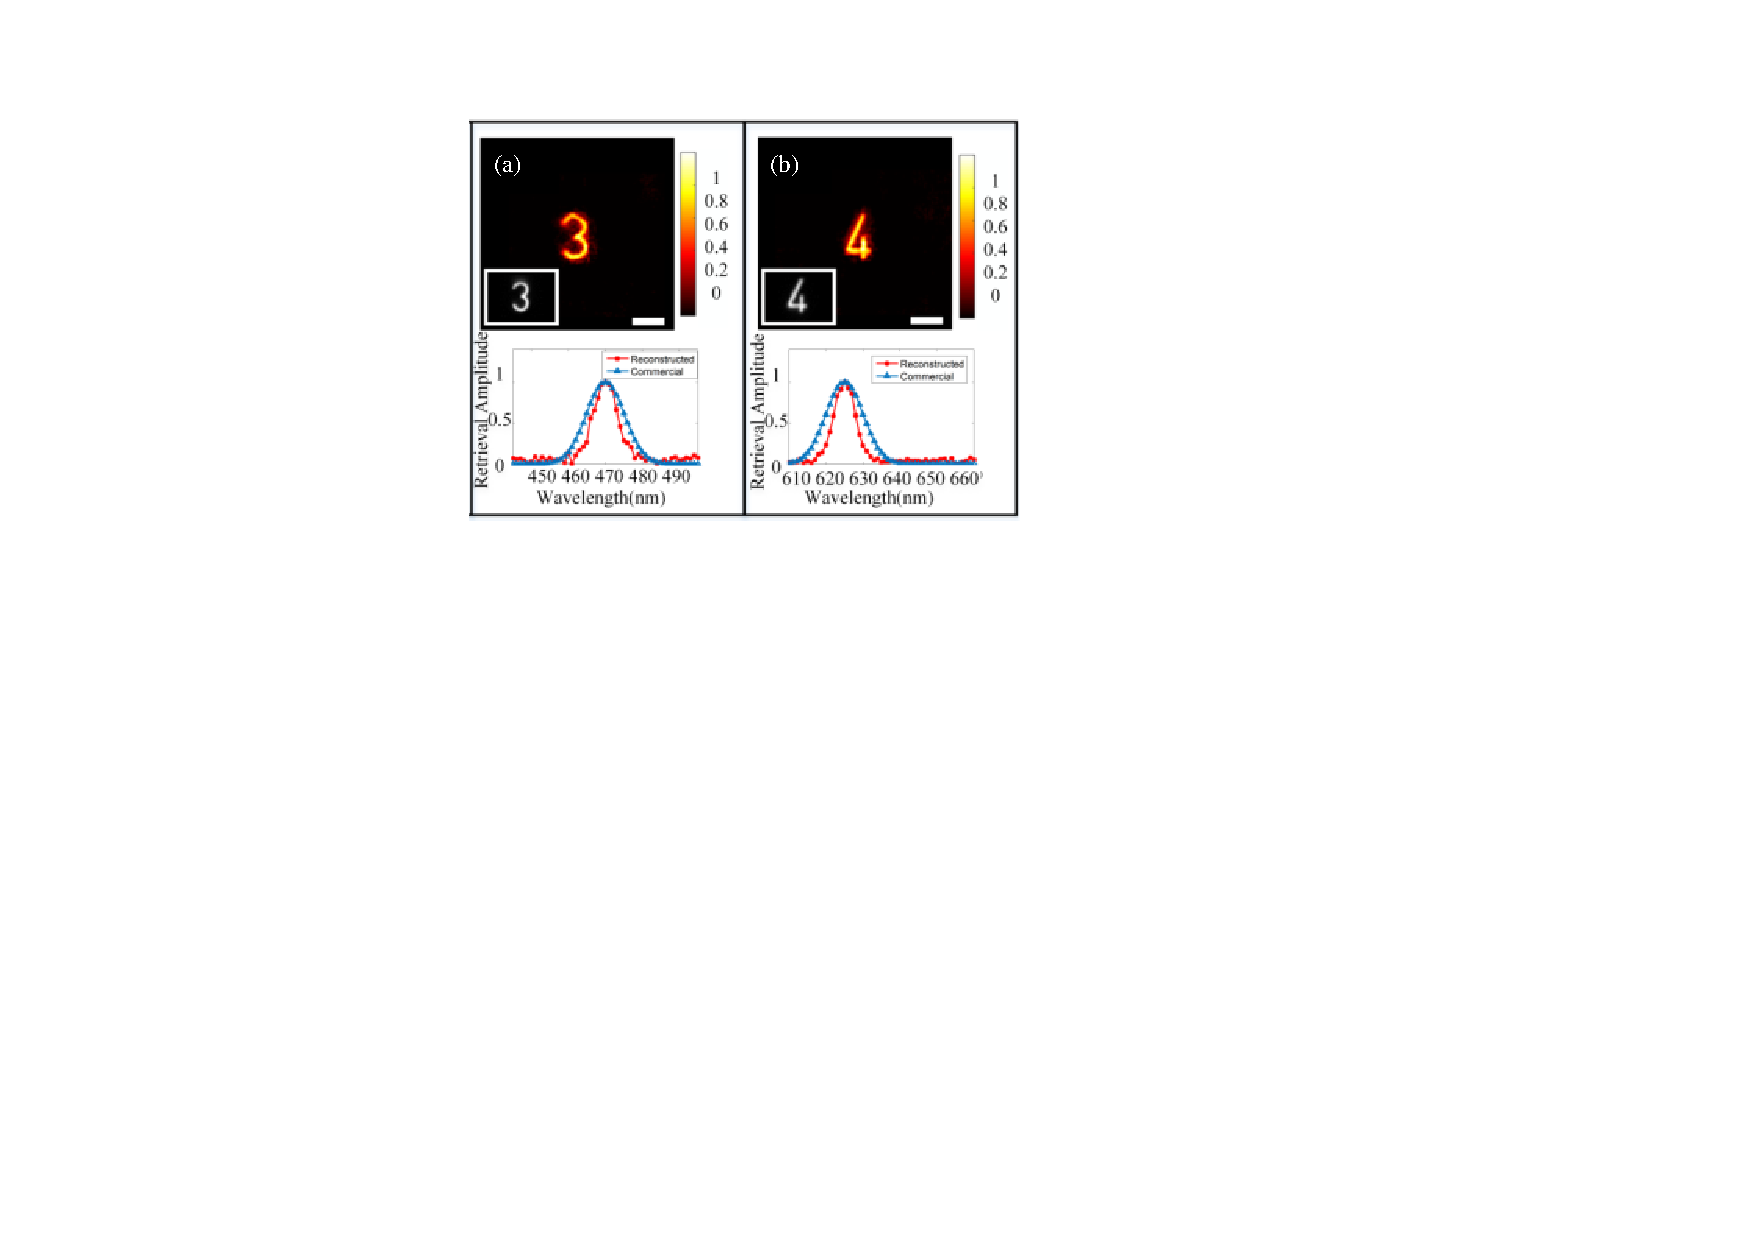
\includegraphics[scale=0.70]{C3.fig12.experimental_setup}
	\caption{宽谱照明时实验结果}
	\label{fig:3.12}
\end{figure}

\subsection{散斑相关成像分析}


\section{声明}

声明是对学位论文创新性和使用授权的声明和说明,论文提交图书馆和存档时作者本人和指导教师必须签名确认。

声明部分标题字体为宋体,字号为四号加粗,居中排列,行距为固定值~20~磅,段落间距为段前~0~磅,段后~0~磅;正文字体为宋体,字号为小四号,行距为固定值~20~磅,段落间距为段前~0~磅,段后~0~磅;标题与正文之间空一行,签名行与正文之间空一行,日期行与签名行之间空一行。

\section{摘要}

摘要是学位论文的内容不加注释和评论的简短陈述,简明扼要陈述学位论文的研究目的、内容、方法、成果和结论,重点突出学位论文的创造性成果和观点。摘要包括中文摘要和英文摘要,硕士学位论文中文摘要字数一般为~1000~字左右,博士学位论文中文摘要字数一般为~1500~字左右。英文摘要内容与中文摘要内容保持一致,翻译力求简明精准。摘要的正文下方需注明论文的关键词,关键词一般为~3~ ~~8~个,关键词和关键词之间用逗号并空一格。

中文摘要标题字体为黑体,字号为三号,居中排列,行距为固定值~20~磅,段落间距为段前~24~磅,段后~18~磅;正文字体为宋体,字号为小四号,行距为固定值~20~磅,段落间距为段前~0~磅,段后~0~ 磅;关键词和正文之间空一行,关键词字体为宋体,字号为小四号,标题加粗。英文摘要标题字体为~Times New Roman~,字号为三号,居中排列,行距为固定值~20~磅,段落间距为段前~24~磅,段后~18~磅;正文的每一段落首行不空格,段落与段落之间空一行;正文字体为~Times New Roman~,字号为小四号,行距为固定值~20~磅,段落间距为段前~0~磅,段后~0~磅;关键词字体为~Times New Roman~,字号为小四号,标题加粗。

\section{插图索引}

学位论文中插图的目录索引。插图索引标题字体为黑体,字号为三号,居中排列,行距为固定值~20~磅,段落间距为段前~24~磅,段后~18~磅;正文内容字体为宋体,字号为小四号,行距为固定值~20~磅,段落间距为段前~0~磅,段后~0~磅。

\section{表格索引}

学位论文中表格的目录索引。表格索引标题字体为黑体,字号为三号,居中排列,行距为固定值~20~磅,段落间距为段前~24~磅,段后~18~磅;正文内容字体为宋体,字号为小四号,行距为固定值~20~磅,段落间距为段前~0~磅,段后~0~磅。

\section{符号对照表}

学位论文中符号代表的意义及单位(或量纲)的说明。符号对照表标题字体为黑体,字号为三号,居中排列,行距为固定值~20~磅,段落间距为段前~24~磅,段后~18~磅;正文内容字体为宋体,字号为小四号,行距为固定值~20~磅。

\section{缩略语对照表}

学位论文中缩略语代表意义的说明。缩略语按照英文单词首字母顺序排列,对照表标题字体为黑体,字号为三号,居中排列,行距为固定值~20~磅,段落间距为段前~24~磅,段后~18~磅;正文内容中文字体为宋体,字号为小四号,英文字体为~Times New Roman~,字号为小四号,行距为固定值~20~磅。

\section{目录}

目录是学位论文的提纲,是论文各组成部分的小标题,应分别依次列出并注明页码。各级标题分别以第一章、~1.1~、~1.1.1~等数字依次标出,目录中最多列出三级标题,正文中如果确需四级标题,用(1)、(2)形式标出。学位论文的前置部分(摘要、插图索引、表格索引、符号对照表、缩略语对照表)和学位论文的主体部分(正文、参考文献、致谢、作者简介)都要在目录中列出。

目录标题字体为黑体,字号为三号,居中排列,行距为固定值~20~磅,段落间距为段前~24~磅,段后~18~磅;目录内容中一级标题字体为黑体,字号为小四号,其余标题字体为宋体,字号为小四号。

\section{正文}

正文是学位论文的主体和核心部分。正文的一级标题居中排列,字体为黑体,字号为三号,行距为固定值~20~磅,段落间距为段前~24~磅,段后~18~磅;二级标题不缩进,字体为宋体加粗,字号为小三号,行距为固定值~20~磅,段落间距为段前~18~磅,段后~12~磅;三级标题缩进~2~ 字符,字体为宋体,字号为四号加粗,行距为固定值~20~磅,段落间距为段前~12~ 磅,段后~6~磅;正文内容字体为宋体,字号为小四号,行距为固定值~20~磅,段落间距为段前~0~磅,段后~0~磅。正文一般包括以下几个方面:

\subsection{绪论}

绪论是学位论文主体部分的开端,切忌与摘要雷同或成为摘要的注解。绪论除了要说明论文的研究目的、研究方法和研究结果外,还应评述与论文研究内容相关的国内外研究现状和相关领域中已有的研究成果;其次还要介绍本项研究工作的前提和任务、理论依据、实验基础、涉及范围、预期结果以及该论文在已有基础上所要解决的问题。

\subsection{各章节}

各章节一般由标题、文字叙述、图、表、公式等构成,章节内容总体要求立论正确,逻辑清晰,数据可靠,层次分明,文字通畅,编排规范。论文中若有与指导教师或他人共同研究的成果,必须明确标注;如果引用他人的结论,必须明确注明出处,并与参考文献保持一致。

(1)图:包括曲线图、示意图、流程图、框图等。图序号一律用阿拉伯数字分章依序编码,如:图~1.3~、图~2.11~。 每一个图应有简短确切的图名,连同图序号置于图的正下方。图名称、图中的内容字号为五号,中文字体为宋体,英文字体为~Times New Roman~,行距一般为单倍行距。图中坐标上标注的符号和缩略词必须与正文保持一致。引用图应在图题右上角标出文献来源;曲线图的纵横坐标必须标注“量、标准规定符号、单位”,这三者只有在不必要标明(如无量纲等)的情况下方可省略。

(2)表:包括分类项目和数据,一般要求分类项目由左至右横排,数据从上到下竖列。分类项目横排中必须标明符号或单位,竖列的数据栏中不要出现“同上”、“同左”等词语,一律要填写具体的数字或文字。表序号一律用阿拉伯数字分章依序编码,如:表~2.5~、表~10.3~。每一个表格应有简短确切的题名,连同表序号置于表的正上方。表名称、表中的内容字号为五号,中文字体为宋体,英文字体为~Times New Roman~,行距一般与正文保持一致。

(3)公式:正文中的公式、算式、方程式等必须编排序号,序号一律用阿拉伯数字分章依序编码,如:(3-32)、 (6-21)。对于较长的公式,另起行居中横排,只可在符号处(如:+、-、*、/、$<$$>$等)转行。公式序号标注于该式所在行(当有续行时,应标注于最后一行)的最右边。连续性的公式在“=”处排列整齐。大于~999~的整数或多于三位的小数,一律用半个阿拉伯数字符的小间隔分开;小于~1~的数应将~0~置于小数点之前。公式的行距一般为单倍行距。

(4)计量单位:学位论文中出现的计量单位一律采用国务院~1984~年~2~月~27~日发布的《中华人民共和国法定计量单位》标准。

\subsection{结论}

结论是学位论文最终和总体的结论,不是正文中各段的小结的简单重复,应准确、精炼、完整,其中要着重阐述作者研究的创造性成果以及在本研究领域中的重大意义,还可提出有待进一步研究和探讨的问题。

\section{参考文献}

参考文献是文中引用的有具体文字来源的文献集合,博士学位论文参考文献一般不少于~80~篇,其中近5年的参考文献不少于~20~篇,硕士学位论文参考文献一般不少于~30~篇,其中近5年的参考文献不少于~5~篇。参考文献标题字体为黑体,字号为三号,居中排列,段落间距为段前~24~磅,段后~18~磅;参考文献若是中文文献,字体为宋体,字号为五号,若是英文文献,字体为~Times New Roman~,字号为五号。学位论文的撰写要本着严谨求实的科学态度,凡有引用他人成果之处,引用处右上角用方括号标注阿拉伯数字编排的序号(必须与参考文献一致),同时所有引用的文献必须用全称,不能缩写,并按论文中所引用的顺序列于文末。引用文献的作者不超过~3~位时全部列出,超过时列前~3~位,后加“等”字或“et al.”。 参考文献的著录要符合《文后参考文献著录规则》(GB/T7714-2005)要求:

(1)期刊(报纸)参考文献:[序号] 主要责任者. 文献名称[文献类别代码]. 期刊(报纸)名, 年份, 卷(期): 引文页码.

(2)专著参考文献:[序号] 主要责任者. 专著名称[文献类别代码]. 其他责任者. 出版地: 出版单位, 出版年份.

(3)专利参考文献:[序号] 主要责任者. 专利名称: 国别, 专利号[文献类别代码]. 出版日期.

(4)技术标准参考文献:[序号] 起草责任者. 标准代号-标准顺序号-发布年. 标准名称[文献类别代码]. 出版地: 出版单位,出版年份.

(5)电子参考文献:[序号] 主要责任者. 题名[文献类别代码]. 获取和访问路径. [引用日期].

(6)会议论文集参考文献:[序号] 编者. 论文集名. (供选择项:会议名, 会址, 开会年)出版地: 出版者, 出版年份.

(7)学位论文参考文献:[序号]  主要责任者. 文献题名[文献类别代码]. 保存地: 保存单位, 年份.

(8)国际、国家标准参考文献:[序号] 标准代号. 标准名称[文献类别代码]. 出版地: 出版者, 出版年.

(9)报告类参考文献:[序号] 主要责任者. 文献题名[文献类别代码]. 报告地: 报告会主办单位, 年份.

参考文献著录中的文献类别代码:

(1)普通图书:M     \par
(2)会议录:C       \par
(3)汇编:G         \par
(4)报纸:N         \par
(5)期刊:J         \par
(6)学位论文:D     \par
(7)报告:R         \par
(8)标准:S         \par
(9)专利:P         \par
(10)数据库:DB     \par
(11)计算机程序:CP \par
(12)电子公告:EB   \par
载体类型:           \par
网络:OL             \par
磁带:MT             \par
磁盘:MK             \par
光盘:CD

\section{致谢}

作者对完成论文提供帮助和支持的组织和个人表示感谢的文字记载。致谢标题字体为黑体,字号为三号,居中排列,行距为固定值~20~磅,段落间距为段前~24~磅,段后~18~磅;正文内容字体为宋体,字号为小四号,行距为固定值~20~磅,段落间距为段前~0~磅,段后~0~磅。

\section{作者简介}

对作者的简要介绍,主要包括个人基本情况、教育背景、攻读博士/硕士学位期间的研究成果等三个部分内容。攻读博士/硕士学位期间的研究成果是指本人攻读博士/硕士学位期间发表(或录用)的学术论文,申请(授权)专利、参与的科研项目及科研获奖等情况,分别按时间顺序列出。其中,发表论文、申请(授权)专利、科研获奖只列出作者排名前~3~名的,参与的科研项目按重要程度最多列出~5~项。作者简介标题字体为黑体,字号为三号,居中排列,行距为固定值~20~ 磅,段落间距为段前~24~磅,段后~18~磅。作者简介的正文内容严格按照本模板中的范例书写。

\section{其他}

学位论文中如果需要注释,可作为脚注在页下分别著录,切忌在文中注释;如果有附录部分,可编写在正文之后,与正文连续编页码,每一附录均另页起,附录依次用大写英文字母~A、B、C……编序号,如:附录~A~、附录~B~等。
